% =============================================================================
%  TIỂU LUẬN
%  Thiết kế và triển khai hệ thống giám sát và điều khiển môi trường trang trại thông minh
%  Sinh viên: [Đã ẩn thông tin]
% =============================================================================
\documentclass[12pt, a4paper]{article}

% =============================================================================
% 1. TIẾNG VIỆT (XeLaTeX) & SIZE 13
% =============================================================================
\usepackage{fontspec}
\usepackage{polyglossia}
\setmainlanguage{vietnamese}
\setotherlanguage{english}

\setmainfont{Times New Roman}

% Để có cỡ chữ 13pt chuẩn
\usepackage{scrextend}
\changefontsizes{13pt}

% =============================================================================
% 2. MARGIN & PAGE
% =============================================================================
\usepackage{geometry}
\geometry{
  a4paper,
  top    = 2.0cm,
  bottom = 2.0cm,
  left   = 3.0cm,
  right  = 2.0cm,
  headheight = 14.5pt
}

\usepackage{setspace}
\onehalfspacing

% =============================================================================
% 3. TIỆN ÍCH
% =============================================================================
\usepackage{hyperref}
\usepackage{graphicx}
% Overleaf/Linux phân biệt hoa thường: thử cả images/ và Images/
\graphicspath{{images/}{Images/}}
\usepackage{float}
\usepackage{booktabs}
\usepackage{array}
\usepackage{tabularx}
% Cột căn giữa / trái (dùng trong tabular, tabularx)
\newcolumntype{C}[1]{>{\centering\arraybackslash}p{#1}}
\newcolumntype{L}[1]{>{\raggedright\arraybackslash}p{#1}}
\usepackage{longtable}
\usepackage{seqsplit}
\usepackage{enumitem}
\usepackage{titlesec}
\usepackage{tocloft}
\usepackage{fancyhdr}
\usepackage{xcolor}
\usepackage{listings}
\usepackage{ifthen}
\usepackage{amssymb}
% notbib: tự thêm mục lục cho thebibliography — ta đã \addcontentsline thủ công
\usepackage[nottoc,notlof,notlot,notbib]{tocbibind}
\usepackage{tikz}

% Cấu hình listings (mã nguồn)
\lstset{
  basicstyle   = \ttfamily\small,
  keywordstyle = \color{blue}\bfseries,
  commentstyle = \color{gray}\itshape,
  stringstyle  = \color{orange},
  breaklines   = true,
  frame        = single,
  numbers      = left,
  numberstyle  = \tiny\color{gray},
  captionpos   = b
}

\lstdefinestyle{ccode}{
    language=C++,
    backgroundcolor=\color{white},
    commentstyle=\color{gray}\itshape,
    keywordstyle=\color{blue}\bfseries,
    stringstyle=\color{orange},
    numberstyle=\tiny\color{gray},
    basicstyle=\ttfamily\small,
    breaklines=true,
    frame=single,
    numbers=left,
    numbersep=5pt,
    stepnumber=1,
    tabsize=4,
    keepspaces=true,
    showstringspaces=false,
    captionpos=b,
    xleftmargin=10pt
}

% JSON (và flow Node-RED): language=Java để listings nhận dạng chuỗi;
% tránh \color{green} (xanh lá chói trên nền trắng) — dùng xanh đậm / tím than.
\lstdefinestyle{jcode}{
    language=Java,
    backgroundcolor=\color{white},
    commentstyle=\color{gray}\itshape,
    keywordstyle=\color{violet!55!black}\bfseries,
    stringstyle=\color{blue!35!black},
    numberstyle=\tiny\color{gray},
    basicstyle=\ttfamily\small,
    breaklines=true,
    frame=single,
    numbers=left,
    numbersep=5pt,
    stepnumber=1,
    tabsize=4,
    keepspaces=true,
    showstringspaces=false,
    captionpos=b,
    xleftmargin=10pt
}

% =============================================================================
% 4. SỐ TRANG (theo rules: chỉ giữa chân trang; không gạch/ngăn/ số ở đầu trang)
% =============================================================================
\fancypagestyle{plain}{%
  \fancyhf{}%
  \fancyfoot[C]{\thepage}%
  \renewcommand{\headrulewidth}{0pt}%
  \renewcommand{\footrulewidth}{0pt}%
}
\pagestyle{fancy}
\fancyhf{}
\fancyhead[L]{}\fancyhead[C]{}\fancyhead[R]{}
\fancyfoot[C]{\thepage}
\renewcommand{\headrulewidth}{0pt}
\renewcommand{\footrulewidth}{0pt}

\hypersetup{
  unicode    = true,
  colorlinks = true,
  linkcolor  = black,
  citecolor  = black,
  urlcolor   = blue
}

% =============================================================================
% 5. ĐỊNH NGHĨA MACRO
% =============================================================================
% \detokenize: cho phép _, {, } trong định danh (vd. WIFI_SSID) mà không gây lỗi math mode
\newcommand{\code}[1]{\texttt{\detokenize{#1}}}
\newcommand{\file}[1]{\textbf{\texttt{\detokenize{#1}}}}
\newcommand{\codebreak}[1]{\texttt{\seqsplit{#1}}}
\renewcommand{\contentsname}{MỤC LỤC}

% =============================================================================
% 6. MACRO ĐÓNG KHUNG VĂN BẢN (theo Nguyễn Thái Sơn)
% =============================================================================
% \khung{độ rộng}{nội dung} — vẽ khung bao quanh đoạn văn bản.
% Ví dụ: \khung{.8\textwidth}{Nội dung cần đóng khung}
\newcommand{\khung}[2]{%
  \hspace*{-.6cm}%
  \begin{tabular}{|l|}
    \hline
    \parbox{#1}{\vphantom{\tiny i}#2} \\
    \hline
  \end{tabular}%
}

% =============================================================================
% ========================  NỘI DUNG TÀI LIỆU  ============================
% =============================================================================
\begin{document}
\setcounter{secnumdepth}{3}
\setcounter{tocdepth}{3}

% =============================================================================
% TRANG BÌA
% =============================================================================
\newgeometry{top=2.0cm, bottom=2.0cm, left=2.0cm, right=2.0cm}
\thispagestyle{empty}
\begin{titlepage}
\begin{tikzpicture}[overlay, remember picture]
  \draw [line width=2pt] ([shift={(2cm,-2cm)}] current page.north west) rectangle ([shift={(-1.5cm,2cm)}] current page.south east);
  \draw [line width=0.5pt] ([shift={(2.1cm,-2.1cm)}] current page.north west) rectangle ([shift={(-1.6cm,2.1cm)}] current page.south east);
\end{tikzpicture}

% --- Phần đầu: trường + logo ---
\begin{center}
  \fontsize{16}{20}\selectfont\bfseries
  BỘ GIÁO DỤC VÀ ĐÀO TẠO\\
  TRƯỜNG ĐẠI HỌC KHOA HỌC\\
  KHOA CÔNG NGHỆ THÔNG TIN\\[0.4cm]
  
\includegraphics[width=4.5cm]{logo.png}
\end{center}

\vspace{1.1cm}

% --- Tiêu đề đề tài (căn giữa, cỡ lớn) ---
\begin{center}
  \fontsize{17}{22}\selectfont\bfseries
  THIẾT KẾ VÀ TRIỂN KHAI HỆ THỐNG\\
  GIÁM SÁT VÀ ĐIỀU KHIỂN MÔI TRƯỜNG\\
  TRANG TRẠI THÔNG MINH
\end{center}

\vspace{1.4cm}

% --- Học phần / mã HP (căn giữa, nhỏ hơn tiêu đề) ---
\begin{center}
  \fontsize{14}{18}\selectfont\bfseries
  TÊN LỚP HỌC PHẦN: PHÁT TRIỂN ỨNG DỤNG IOT\\[0.45cm]
  MÃ HỌC PHẦN: 2025-2026.2.TIN4024.009\\[0.45cm]
  GIẢNG VIÊN HƯỚNG DẪN: TS. LÊ HỮU BÌNH
\end{center}

\vfill

\vspace{2.2cm}

\begin{center}
  {\large Huế, Ngày 08 Tháng 04 Năm 2026}
\end{center}

\end{titlepage}
\restoregeometry
\newpage

% =============================================================================
% LỜI CẢM ƠN
% =============================================================================
\thispagestyle{empty}
\vspace*{0.4cm}
\begin{center}
  \fontsize{17}{21}\selectfont\bfseries LỜI CẢM ƠN\par
  \vspace{0.2ex}
  \rule{0.28\textwidth}{1.8pt}
\end{center}
\vspace{0.6cm}

\parindent=1.1cm
\setlength{\parskip}{0.55ex plus 0.2ex}

Lời đầu tiên, em xin gửi lời cảm ơn sâu sắc đến Khoa Công nghệ Thông tin – Trường Đại học Khoa học – Đại học Huế, nơi đã tạo điều kiện thuận lợi và môi trường học tập tuyệt vời để em có cơ hội tham gia và hoàn thành bài tiểu luận này. Sự hỗ trợ từ phía nhà trường đã giúp em không chỉ phát triển kiến thức chuyên môn mà còn rèn luyện được những kỹ năng cần thiết để chuẩn bị cho tương lai.

Đặc biệt, em xin bày tỏ lòng biết ơn chân thành đến TS. Lê Hữu Bình, người đã tận tình hướng dẫn, chia sẻ kinh nghiệm và truyền đạt những kiến thức quý báu trong suốt quá trình em thực hiện bài tiểu luận. Những lời chỉ bảo tận tình và sự quan tâm của thầy đã giúp em vượt qua những khó khăn và hoàn thành bài tiểu luận một cách tốt nhất. Em cảm thấy may mắn và trân quý những lời khuyên, sự giúp đỡ từ thầy, người đã luôn kiên nhẫn đồng hành cùng em qua từng bước đi.

Bên cạnh đó, em xin gửi lời tri ân đến toàn thể quý thầy cô của Khoa Công nghệ Thông tin – Trường Đại học Khoa học – Đại học Huế, những người đã không quản ngại khó khăn, luôn tận tâm truyền đạt kiến thức, dạy bảo và hỗ trợ em trong suốt thời gian học tập tại trường. Sự tận tụy và cống hiến của quý thầy cô không chỉ giúp em đạt được thành tích học tập mà còn giúp em nhận thức rõ ràng về con đường sự nghiệp mà em đang theo đuổi.

Xin trân trọng cảm ơn!

\parindent=0pt
\parskip=0pt
\vspace{0.5cm}
\hfill\begin{minipage}[t]{7cm}
  \fontsize{13}{17}\selectfont
  \begin{flushright}
    Huế, tháng 04 năm 2026
  \end{flushright}
\end{minipage}

\newpage

% =============================================================================
% DANH MỤC TỪ VIẾT TẮT
% =============================================================================
\thispagestyle{empty}
\vspace*{0.4cm}
\begin{center}
  \fontsize{17}{21}\selectfont\bfseries DANH MỤC CÁC TỪ VIẾT TẮT
\end{center}
\vspace{0.5cm}

\noindent
\begingroup
\renewcommand{\arraystretch}{1.2}%
\begin{tabularx}{\textwidth}{@{}C{2.5cm}X@{}}
  \toprule
  \textbf{Ký hiệu} & \textbf{Giải thích} \\
  \midrule
  \textbf{API}   & Application Programming Interface --- Giao diện lập trình ứng dụng \\
  \textbf{DHT}    & Digital Humidity and Temperature --- Cảm biến nhiệt độ và độ ẩm số \\
  \textbf{GPIO}   & General Purpose Input/Output --- Chân vào/ra đa mục đích \\
  \textbf{IoT}    & Internet of Things --- Internet vạn vật \\
  \textbf{JSON}   & JavaScript Object Notation --- Định dạng chuỗi dữ liệu khóa-giá trị \\
  \textbf{LED}    & Light-Emitting Diode --- Điốt phát quang \\
  \textbf{MQTT}   & Message Queuing Telemetry Transport --- Giao thức truyền thông pub/sub \\
  \textbf{MQTT Broker} & Phần mềm trung gian nhận và phân phối message theo topic \\
  \textbf{NRD}    & Node-RED Dashboard --- Giao diện Dashboard của Node-RED \\
  \textbf{Pub/Sub} & Publisher/Subscriber --- Mô hình gửi/nhận message qua topic \\
  \textbf{TLS}    & Transport Layer Security --- Giao thức bảo mật tầng truyền tải \\
  \bottomrule
\end{tabularx}
\endgroup

\newpage

% =============================================================================
% MỤC LỤC
% =============================================================================
\pagenumbering{gobble}
\thispagestyle{empty}
\vspace*{0.35\baselineskip}
{\setstretch{1}\normalsize
  \tableofcontents
}
\newpage

% =============================================================================
% BẮT ĐẦU ĐÁNH SỐ TRANG
% =============================================================================
\pagenumbering{arabic}
\thispagestyle{fancy}
\fontsize{13}{19.5}\selectfont

% =============================================================================
% PHẦN MỞ ĐẦU (theo bố cục Phụ lục II)
% =============================================================================
% =============================================================================
% 1. ĐẶT VẤN ĐỀ
% =============================================================================
\section*{CHƯƠNG 1: ĐẶT VẤN ĐỀ}
\phantomsection
\addcontentsline{toc}{section}{CHƯƠNG 1: ĐẶT VẤN ĐỀ}
\label{sec:ch1}
\setcounter{section}{1}
\setcounter{subsection}{0}

\subsection{Bối cảnh và tính cấp thiết của đề tài}
Trong bối cảnh biến đổi khí hậu diễn biến phức tạp và quá trình đô thị hóa diễn ra nhanh chóng, việc áp dụng công nghệ thông minh vào sản xuất nông nghiệp ngày càng trở nên quan trọng và thực tiễn. Hiện nay, phương pháp tưới tiêu thủ công tại các mô hình nhà kính, trang trại vừa và nhỏ, hay quy mô hộ gia đình (sân thượng, ban công) thường bộc lộ nhiều hạn chế, tốn kém thời gian và khó đảm bảo cung cấp nước đúng mức độ, đúng thời điểm. Những khó khăn này đặt ra nhu cầu lớn trong việc ứng dụng Internet of Things (IoT) để chuyển đổi số nông nghiệp. 

Việc trang bị một hệ thống có khả năng tự động theo dõi xuyên suốt các thông số thiết yếu (nhiệt độ, độ ẩm không khí, độ ẩm của đất) kết hợp với chức năng cảnh báo sớm và điều khiển bơm tưới tiêu từ xa là một tiện ích không thể thiếu. Tính năng tự động hóa giám sát — publish dữ liệu lên MQTT Cloud Broker — cập nhật lên giao diện trực quan (Dashboard) và thực hiện subscribe các lệnh điều khiển ngược trở lại cho thiết bị phần cứng chính là hướng tiếp cận hiệu quả nhằm giải quyết nhu cầu hiển hiện trên. Đồng thời, đây cũng là hướng đi bám sát với mục đích và nội dung cốt lõi mong đợi của học phần Phát triển Ứng dụng IoT.

\subsection{Mục tiêu thiết kế và phạm vi nghiên cứu}
Đề tài tập trung thiết kế và triển khai một hệ thống mô phỏng quy trình giám sát và điều khiển trang trại thông minh cỡ nhỏ. Các mục tiêu kỹ thuật cụ thể được giới hạn trong phạm vi thực thi thống nhất giữa Firmware và Flow điều khiển như sau:

\begin{itemize}
  \item Đọc nhiệt độ, độ ẩm không khí (DHT22, GPIO 4) và độ ẩm đất mô phỏng bằng biến trở (ADC GPIO 34), chu kỳ 5 giây.
  \item Publish dữ liệu JSON lên MQTT Broker (HiveMQ Cloud) qua giao thức TLS (cổng 8883), topic \code{iot/farm/sensor}; đồng thời subscribe để nhận lệnh điều khiển tại topic \code{iot/farm/control}.
  \item Điều khiển LED mô phỏng máy bơm (GPIO 5), cảnh báo buzzer (GPIO 18) khi đất khô (ngưỡng raw ADC $<$ 2048 trong code).
  \item Node-RED Dashboard: gauge, biểu đồ, toast cảnh báo, nút bơm thủ công và chế độ tưới tự động theo \file{node-red.json}.
\end{itemize}

% =============================================================================
% 2. NỘI DUNG THỰC HIỆN (mục lục chi tiết; nội dung khớp main.cpp / node-red.json)
% =============================================================================
\section*{CHƯƠNG 2: NỘI DUNG THỰC HIỆN}
\phantomsection
\addcontentsline{toc}{section}{CHƯƠNG 2: NỘI DUNG THỰC HIỆN}
\label{sec:ch2}
\setcounter{section}{2}
\setcounter{subsection}{0}

\subsection{Thu thập dữ liệu môi trường (DHT22 và độ ẩm đất)}

Firmware định kỳ 5 giây (\code{PUBLISH_INTERVAL}) gọi \code{readSensor()}: đọc nhiệt độ và độ ẩm không khí qua thư viện DHT trên GPIO \code{DHT_PIN} (4), đọc độ ẩm đất thô qua \code{analogRead(SOIL_PIN)} với \code{SOIL_PIN} = 34 (ADC 12-bit, 0--4095). Nếu DHT trả NaN, giá trị được thay bằng số ngẫu nhiên trong khoảng an toàn để hệ không dừng (\file{main.cpp}).

DHT22 đo KK theo giao tiếp 1-wire; độ chính xác tốt hơn DHT11. Potentiometer mô phỏng cảm biến độ ẩm đất: giá trị ADC càng thấp thì trên Dashboard (công thức \code{(1 - soil/4095)*100}) đất càng khô.

\begin{figure}[H]
  \centering
  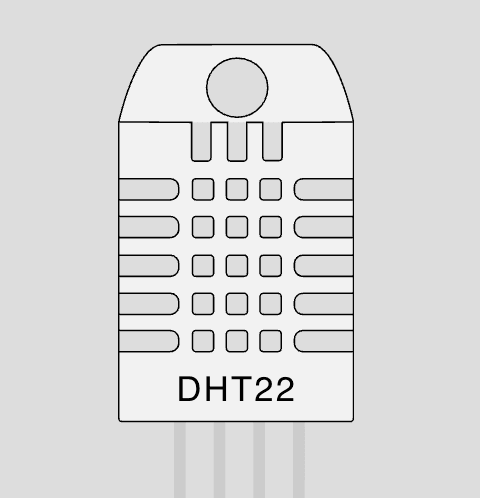
\includegraphics[width=0.22\linewidth]{dht22.png}
  \caption{Cảm biến DHT22 đo đạc thông số nhiệt độ và độ ẩm không khí}
  \label{fig:2_dht22}
\end{figure}

\subsection{Chỉ báo cục bộ: LED mô phỏng máy bơm và buzzer cảnh báo}

GPIO \code{LED_PIN} (5) điều khiển LED cực dương (mô phỏng máy bơm). GPIO \code{BUZZER_PIN} (18) dùng PWM qua \code{ledc} trong hàm \code{toneBuzzer()}: khi \code{soilRaw < 2048}, firmware phát cảnh báo 2\,kHz trong 300\,ms mỗi chu kỳ đọc (\file{main.cpp}).

\begin{figure}[H]
  \centering
  \begin{minipage}{0.45\textwidth}
    \centering
    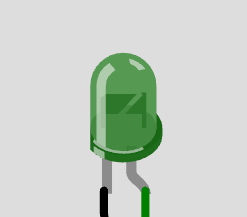
\includegraphics[width=0.45\linewidth]{led.png}
    \caption{Đèn LED mô phỏng máy bơm}
    \label{fig:2_led}
  \end{minipage}\hfill
  \begin{minipage}{0.45\textwidth}
    \centering
    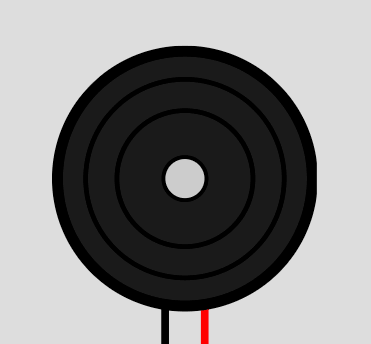
\includegraphics[width=0.45\linewidth]{buzzer.png}
    \caption{Còi Buzzer phát âm thanh cảnh báo}
    \label{fig:2_buzzer}
  \end{minipage}
\end{figure}

\subsection{Truyền dữ liệu qua MQTT (HiveMQ Cloud, TLS)}

MQTT (Message Queuing Telemetry Transport) là giao thức truyền thông nhẹ, được thiết kế đặc biệt cho các thiết bị IoT có băng thông thấp, năng lượng hạn chế hoặc kết nối không ổn định. MQTT hoạt động theo mô hình publisher/subscriber (pub/sub), trong đó thiết bị gửi (publisher) thực hiện publish dữ liệu lên một topic trên MQTT Broker, và các thiết bị nhận (subscriber) sẽ subscribe vào các topic tương ứng để nhận dữ liệu. Mô hình này tách biệt người gửi và người nhận, giúp hệ thống dễ mở rộng.

MQTT sử dụng cơ chế QoS (Quality of Service) với ba mức: QoS 0 (At most once) — message được publish một lần, không xác nhận; QoS 1 (At least once) — gửi ít nhất một lần, có xác nhận, đảm bảo message đến; QoS 2 (Exactly once) — đảm bảo message đến đúng một lần, phù hợp cho các ứng dụng yêu cầu độ tin cậy cao. Trong đề tài này, QoS 0 được sử dụng cho cả việc publish dữ liệu cảm biến (\code{iot/farm/sensor}) và điều khiển (\code{iot/farm/control}), phù hợp với tần suất dữ liệu không quá cao.

HiveMQ Cloud là dịch vụ MQTT Broker dạng cloud do HiveMQ cung cấp, hỗ trợ giao thức bảo mật TLS (Transport Layer Security) trên cổng 8883, đảm bảo dữ liệu truyền giữa thiết bị và broker được mã hóa end-to-end. HiveMQ Cloud có gói miễn phí (Free Tier) cho phép kết nối tối đa 100 thiết bị, đủ cho các ứng dụng demo và học tập.

Cấu hình MQTT trong đề tài:

\begin{itemize}
  \item Broker: \codebreak{b1c8f2cc5cd4416fb74b671a407dc0ff.s1.eu.hivemq.cloud}
  \item Port: \textbf{8883} (TLS)
  \item Protocol: MQTT v3.1.1
  \item Topic gửi dữ liệu cảm biến: \code{iot/farm/sensor}
  \item Topic nhận lệnh điều khiển: \code{iot/farm/control}
\end{itemize}

Lưu ý: topic \code{iot/farm/sensor} và \code{iot/farm/control} được đặt theo chuẩn để dễ mở rộng. Trên ESP32, client dùng \code{WiFiClientSecure} với TLS (cổng \code{MQTT_PORT} = 8883), \code{PubSubClient} publish/subscribe tương ứng (\file{main.cpp}).

\subsection{Xử lý dữ liệu bằng Node-RED}

Node-RED là công cụ lập trình flow-based; dữ liệu từ ESP32 được mô tả chi tiết trong \file{node-red.json}. Message MQTT từ topic \code{iot/farm/sensor} vào node \textbf{mqtt in} rồi phân nhánh song song.

Nhánh thứ nhất (\textbf{Gauge nhiệt độ}): message được chuyển qua node function trích giá trị \code{msg.payload.temperature}, chuyển thành số thực, rồi truyền tới node \textbf{ui\_gauge} để hiển thị kim đồng hồ đo nhiệt độ với ba vùng màu (xanh: bình thường, vàng: trung gian, đỏ: nguy hiểm).

Nhánh thứ hai (\textbf{Gauge độ ẩm không khí}): tương tự, trích giá trị \code{msg.payload.humidity}, truyền tới node \textbf{ui\_gauge} (dạng donut) hiển thị độ ẩm không khí trong nhóm \textbf{Độ ẩm KK}.

Nhánh thứ ba (\textbf{Gauge độ ẩm đất}): trích giá trị \code{msg.payload.soil} từ potentiometer (raw ADC 0–4095), chuyển đổi thành phần trăm \code{Math.round((1 - soil / 4095) * 100)}, truyền tới node \textbf{ui\_gauge} dạng donut với ba vùng màu (đỏ: khô, vàng: trung bình, xanh: ẩm).

Nhánh thứ tư (\textbf{Chart nhiệt độ}): trích giá trị nhiệt độ, gán topic \code{Nhiệt độ °C}, truyền tới node \textbf{ui\_chart} (line chart) để vẽ đồ thị theo thời gian thực, tự động xóa điểm cũ sau 1 giờ (\code{removeOlderUnit: 3600}).

Nhánh thứ năm (\textbf{Chart độ ẩm KK}): trích giá trị độ ẩm không khí, gán topic \code{Độ ẩm KK \%}, truyền tới node \textbf{ui\_chart} để vẽ đồ thị.

Nhánh thứ sáu (\textbf{Chart độ ẩm đất}): trích giá trị độ ẩm đất (đã chuyển \%), gán topic \code{Độ ẩm đất \%}, truyền tới node \textbf{ui\_chart} để vẽ đồ thị.

Nhánh thứ bảy (\textbf{Cảnh báo nhiệt độ cao}): switch node kiểm tra \code{payload.temperature > 35}. Nếu đúng, function node tạo message cảnh báo, truyền tới node \textbf{ui\_toast} hiển thị thông báo ở góc dưới bên trái Dashboard trong 8 giây.

Nhánh thứ tám (\textbf{Cảnh báo độ ẩm KK thấp}): switch node kiểm tra \code{payload.humidity < 40}. Nếu đúng, function node tạo message cảnh báo kèm gợi ý tưới, truyền tới toast.

Nhánh thứ chín (\textbf{Cảnh báo đất khô}): switch node kiểm tra \code{payload.soil < 2048}. Nếu đúng, function node tạo toast thông báo đất khô kèm giá trị phần trăm.

Nhánh thứ mười (\textbf{Cảnh báo nguy hiểm — đất rất khô}): switch node kiểm tra \code{payload.soil < 1024} (dưới 25\% độ ẩm), hiển thị cảnh báo đỏ trên Dashboard (bổ sung cho nhánh 9; buzzer trên ESP32 trong \file{main.cpp} chỉ theo ngưỡng \code{soilRaw < 2048}, không tách thêm ngưỡng 1024).

Nhánh thứ mười một (\textbf{Tưới tự động}): switch node kiểm tra độ ẩm đất $<$ 2048 đồng thời \code{flow.manual == true} (switch \textit{Tưới tự động} trên Dashboard gán biến flow tên \code{manual} --- trùng tên với file \file{node-red.json}). Nếu thỏa điều kiện, change node tạo cấu trúc JSON \code{\{"pump":true,"duration":5\}} và publish thông qua node \textbf{mqtt out} đến topic \code{iot/farm/control}.

\begin{figure}[H]
  \centering
  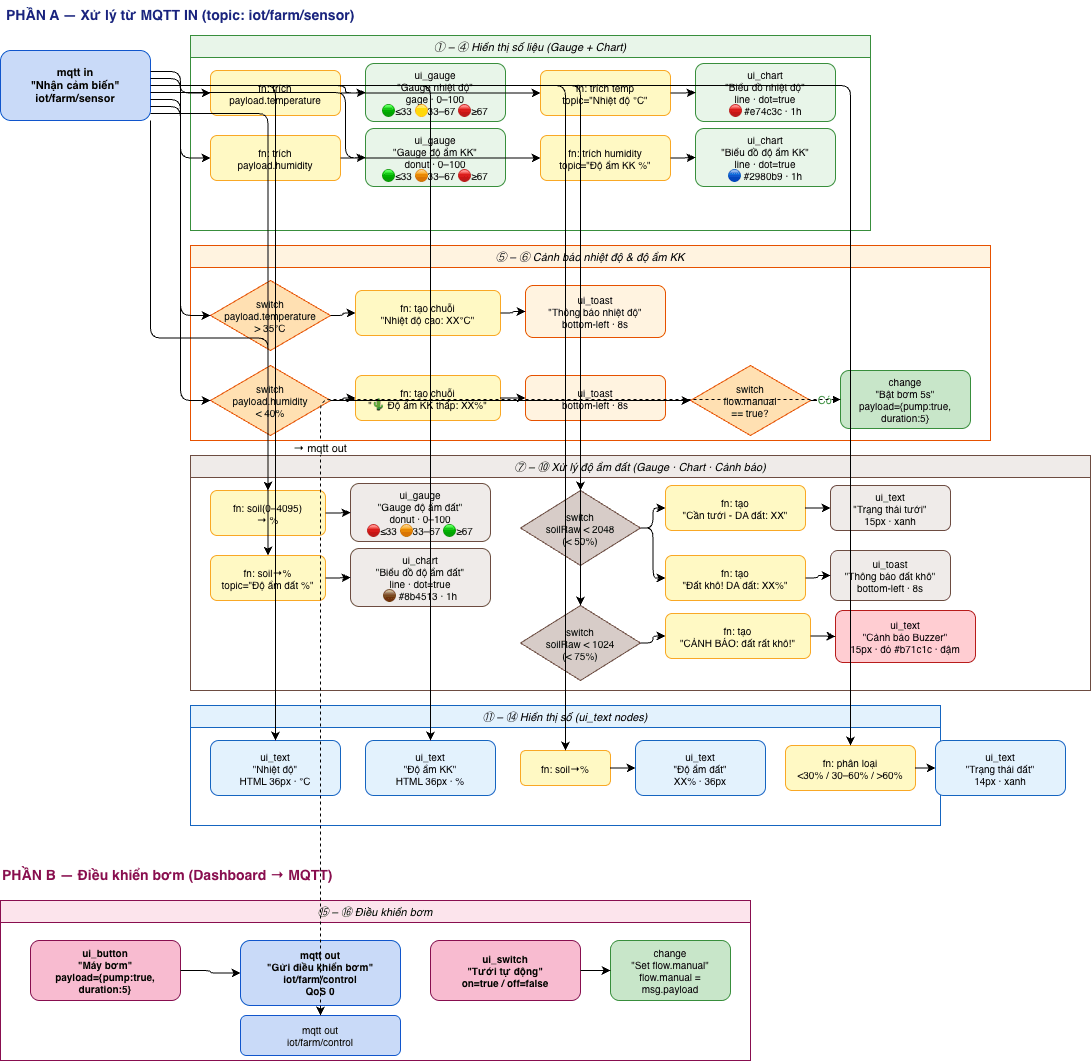
\includegraphics[width=0.9\linewidth]{so-do-flow-nodered.png}
  \caption{Sơ đồ flow xử lý dữ liệu trên Node-RED}
  \label{fig:flow}
\end{figure}

\subsection{Hiển thị dữ liệu trên Dashboard}

Node-RED Dashboard cung cấp các widget: gauge (nhiệt độ, độ ẩm KK, độ ẩm đất), chart đường theo thời gian thực, text trạng thái, nút \textbf{Máy bơm}, switch \textbf{Tưới tự động}, toast cảnh báo. Giao diện truy cập tại \url{http://localhost:1880/ui} (hoặc \url{http://127.0.0.1:1880/ui}).

\begin{figure}[H]
  \centering
  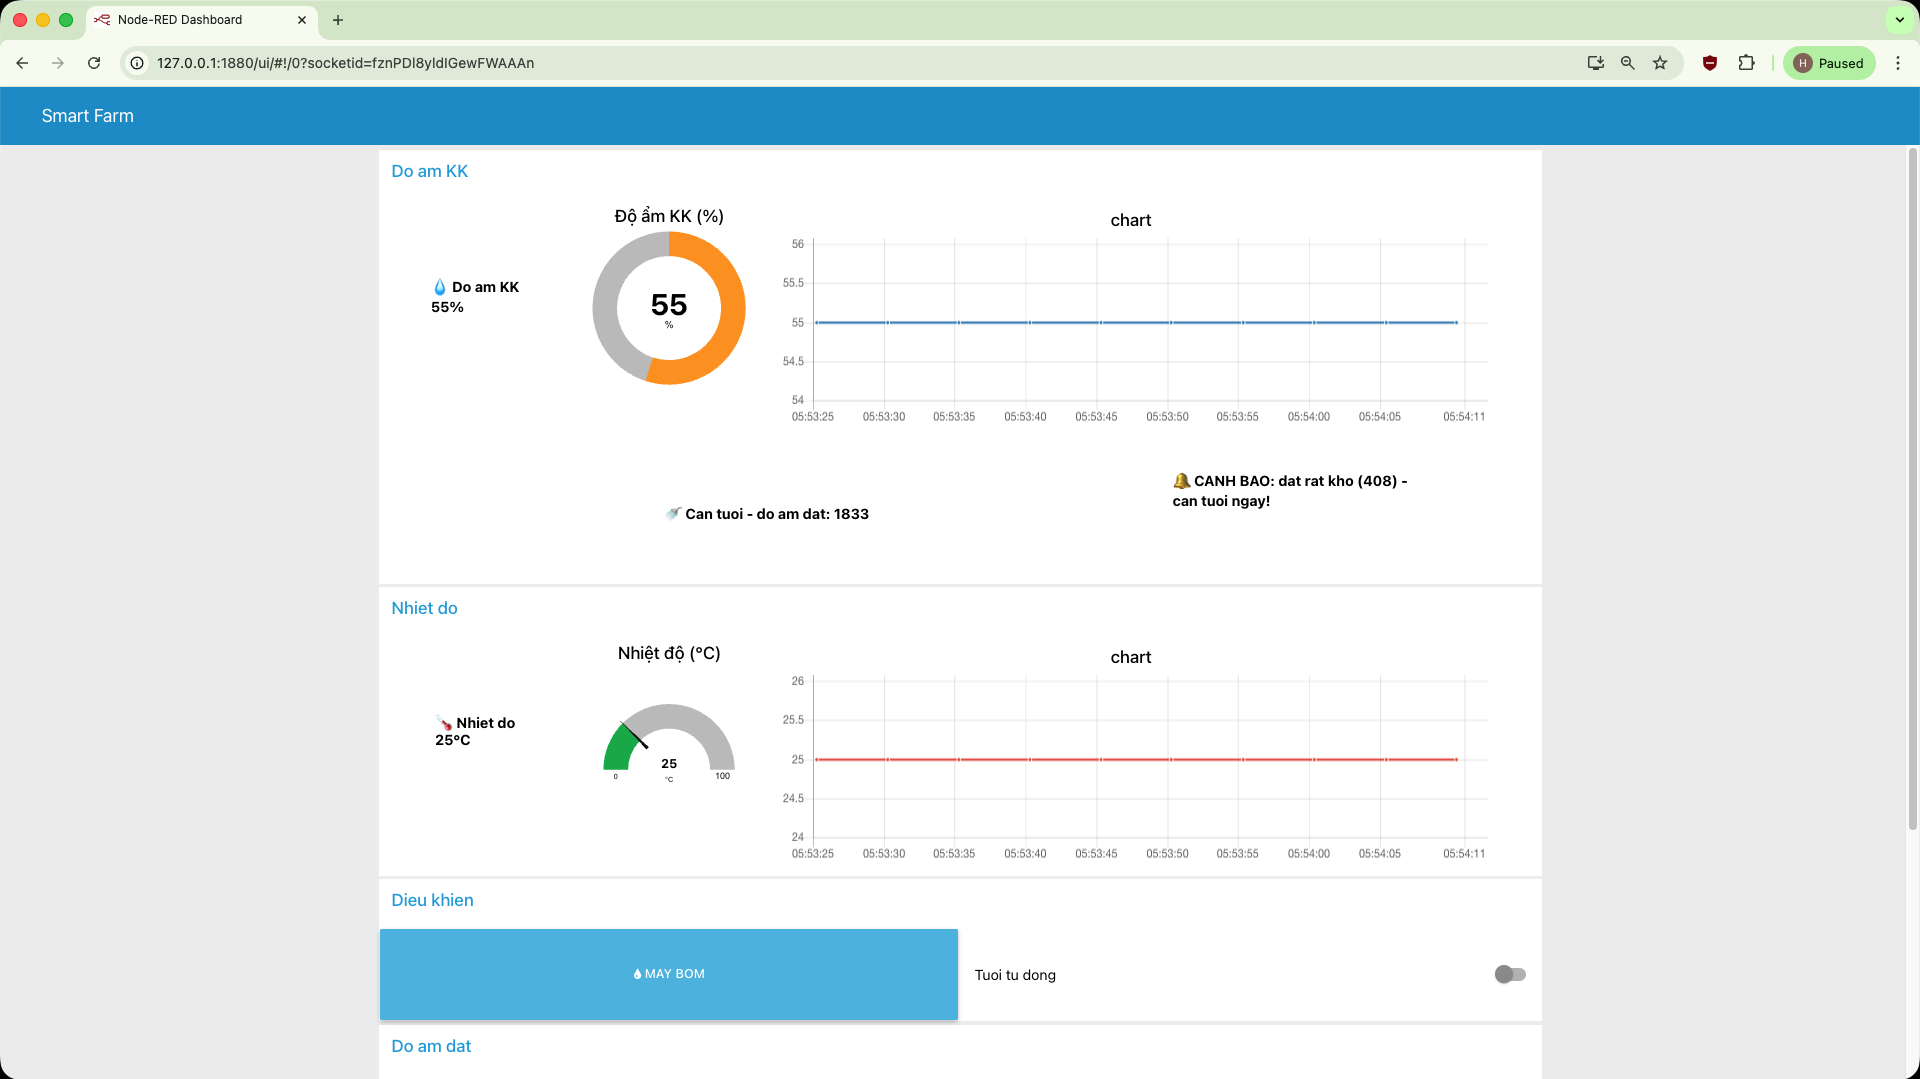
\includegraphics[width=0.9\linewidth]{nodered-dashboard-full-1.png}
  \caption{Giao diện tổng quan hiển thị dữ liệu trên Node-RED Dashboard}
  \label{fig:dashboard-1}
\end{figure}

\subsection{Cảnh báo môi trường}

Trên Dashboard: toast khi \code{temperature > 35}, khi \code{humidity < 40}, khi \code{soil < 2048}, và cảnh báo đỏ khi \code{soil < 1024} (\file{node-red.json}). Trên ESP32: buzzer chỉ phụ thuộc \code{soilRaw < 2048} trong \code{loop()} (không có ngưỡng 1024 riêng trên firmware).

\begin{figure}[H]
  \centering
  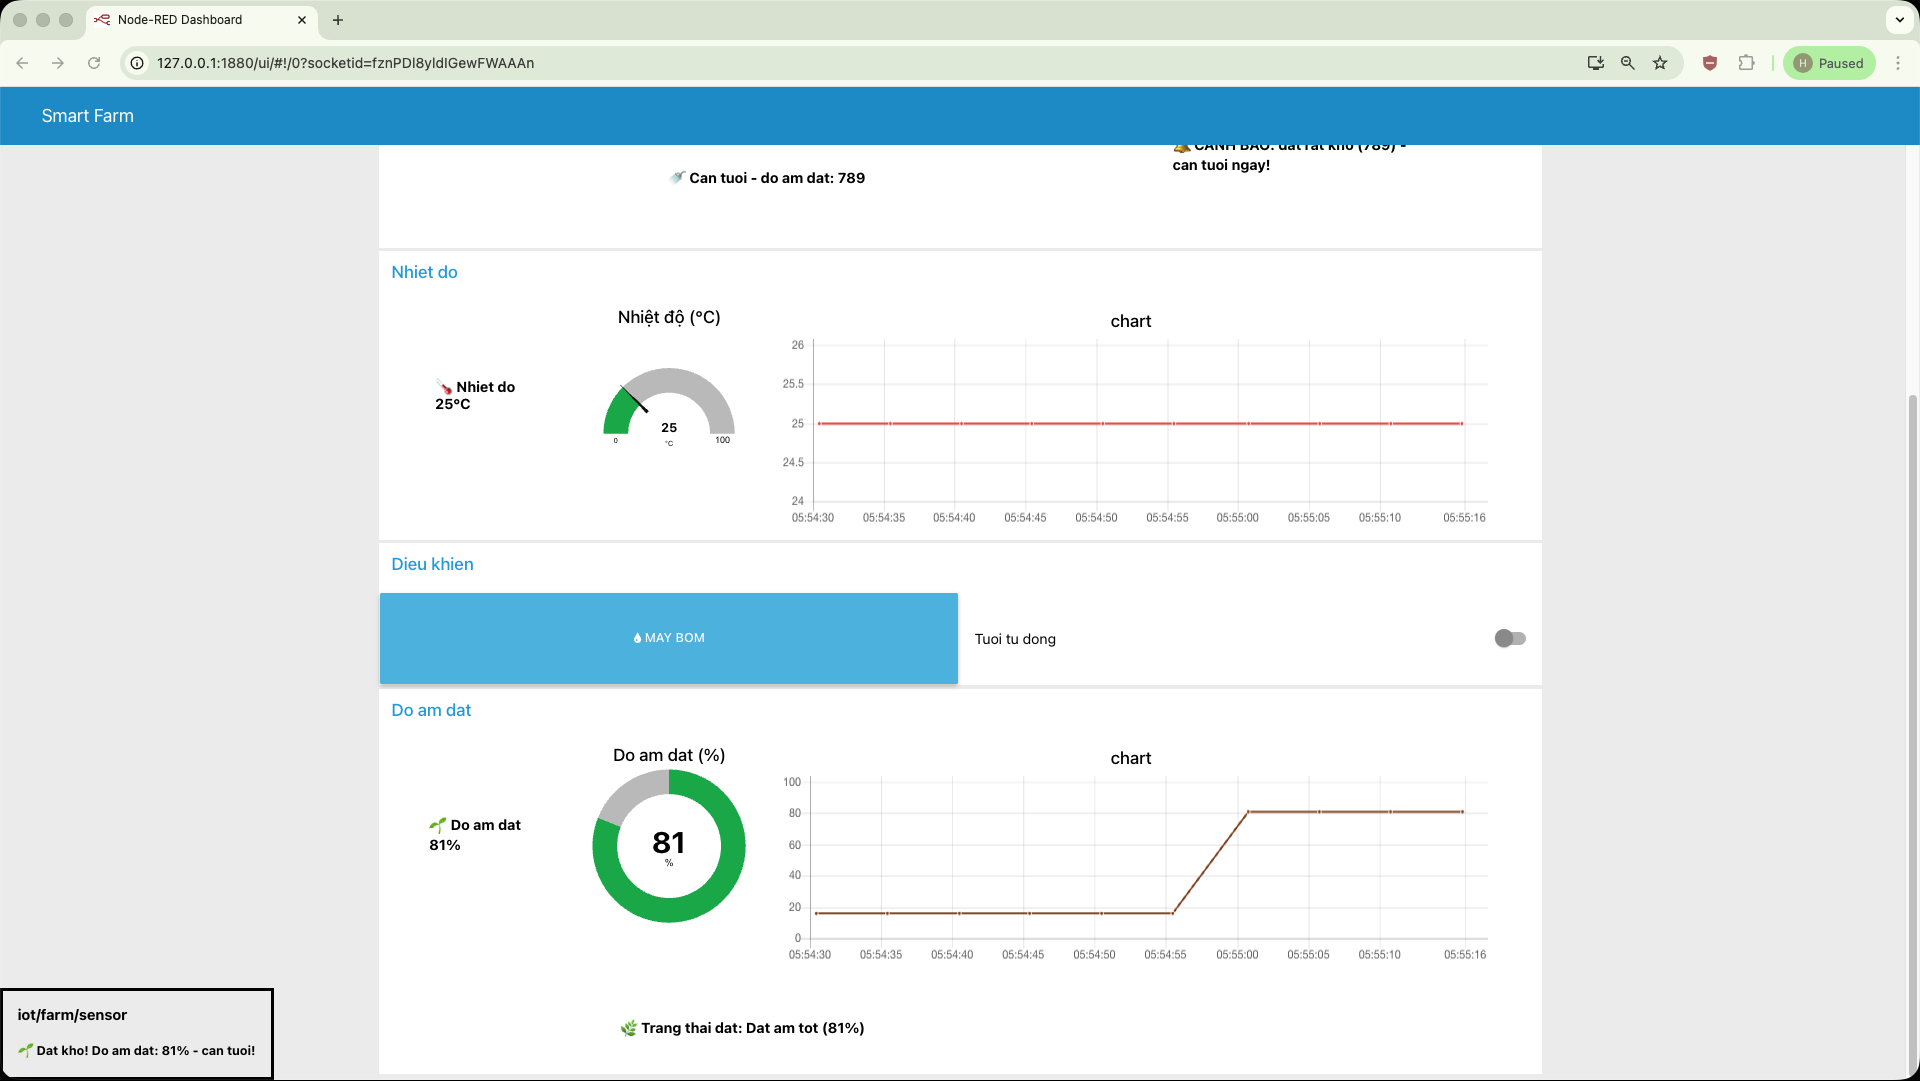
\includegraphics[width=0.9\linewidth]{nodered-dashboard-full-2.png}
  \caption{Giao diện cảnh báo môi trường trên Node-RED Dashboard}
  \label{fig:dashboard-2}
\end{figure}

\subsection{Điều khiển máy bơm từ xa qua MQTT}

Hệ thống cung cấp khả năng điều khiển thiết bị chấp hành thông qua các bản tin định hướng từ máy chủ. Cụ thể, thiết bị ESP32 thực hiện subscribe vào topic điều khiển \code{iot/farm/control} để chờ nhận lệnh. Khi nhận được một gói tin JSON chứa chỉ thị kích hoạt máy bơm, bộ vi xử lý sẽ tiến hành parse dữ liệu và thực thi việc bật cơ cấu chấp hành (mô phỏng bằng đèn LED). Để đảm bảo an toàn và tiết kiệm tài nguyên, hệ thống tích hợp cơ chế tự động ngắt sau một khoảng thời gian vận hành dự kiến. Quy trình này giúp duy trì sự đồng bộ giữa trạng thái hiển thị trên Dashboard và hoạt động thực tế của thiết bị, đồng thời bảo vệ hệ thống khỏi các lỗi vận hành kéo dài không mong muốn.

\begin{figure}[H]
  \centering
  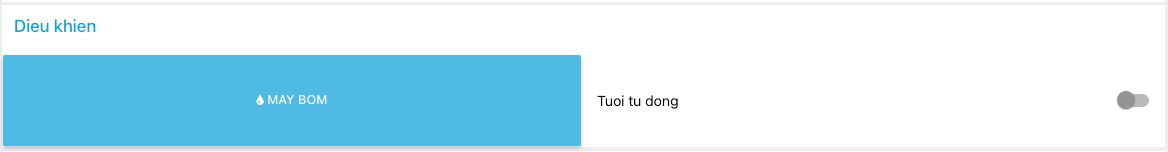
\includegraphics[width=0.9\linewidth]{dieukhien.png}
  \caption{Giao diện nút nhấn và công tắc điều khiển máy bơm từ xa}
  \label{fig:dieukhien}
\end{figure}

\subsection{Duy trì kết nối và đồng bộ trạng thái bơm}

Hệ thống được thiết kế để tự động giám sát và duy trì tính ổn định của các kết nối mạng. Trong vòng lặp chính của chương trình, vi điều khiển liên tục kiểm tra trạng thái của Wi-Fi và giao thức MQTT. Nếu phát hiện sự cố ngắt kết nối, quy trình tái lập liên kết sẽ được thực hiện định kỳ cho đến khi thông tin giao tiếp được khôi phục. Đồng thời, cơ chế giám sát thời gian vận hành máy bơm cũng được thực thi song song để đảm bảo thiết bị tự động ngắt sau một khoảng thời gian quy định, giữ cho trạng thái thực tế luôn khớp với lệnh điều khiển đã gửi.

\subsection{Tự động tưới theo ngưỡng độ ẩm đất (Node-RED)}

Hệ thống tích hợp logic điều khiển tự động dựa trên sự kết hợp giữa các thông số cảm biến thực tế và thiết lập từ người dùng. Khi chế độ tưới tự động được kích hoạt trên Dashboard, hệ thống sẽ liên tục đánh giá giá trị độ ẩm đất đo được. Nếu độ ẩm giảm xuống dưới ngưỡng khô hạn đã thiết lập, Node-RED sẽ tự động tạo và publish các payload điều khiển qua giao thức MQTT để kích hoạt máy bơm nước tưới bù độ ẩm, đảm bảo duy trì môi trường lý tưởng cho cây trồng.

% =============================================================================
% 3. THIẾT KẾ MẠCH IOT
% =============================================================================
\section*{CHƯƠNG 3: THIẾT KẾ MẠCH IoT}
\phantomsection
\addcontentsline{toc}{section}{CHƯƠNG 3: THIẾT KẾ MẠCH IoT}
\label{sec:ch3}
\setcounter{section}{3}
\setcounter{subsection}{0}

\subsection{Thành phần phần cứng}

Hệ thống sử dụng các linh kiện điện tử cơ bản và phổ biến, được lựa chọn nhằm tối ưu chi phí nhưng vẫn đảm bảo độ tin cậy trong việc thu thập dữ liệu và cảnh báo. Các thành phần chính bao gồm:
\begin{itemize}
    \item \textbf{Vi điều khiển trung tâm:} ESP32 DevKit C v4 đóng vai trò bộ não xử lý, kết nối mạng Wi-Fi và giao tiếp MQTT.
    \item \textbf{Cảm biến môi trường:} Cảm biến DHT22 dùng để đo nhiệt độ và độ ẩm không khí với sai số thấp.
    \item \textbf{Cảm biến đo lường (mô phỏng):} Biến trở (Potentiometer) được sử dụng để giả lập tín hiệu điện áp tương tự (ADC) của cảm biến đo độ ẩm đất trong thực tế.
    \item \textbf{Cơ cấu chấp hành và cảnh báo:} Đèn LED (kèm điện trở hạn dòng) giả lập trạng thái hoạt động của máy bơm nước. Còi loa (Buzzer) điều khiển bằng xung PWM nhằm phát âm thanh báo động cường độ cao khi đất quá khô.
\end{itemize}

\begin{figure}[H]
  \centering
  \begin{minipage}{0.45\textwidth}
    \centering
    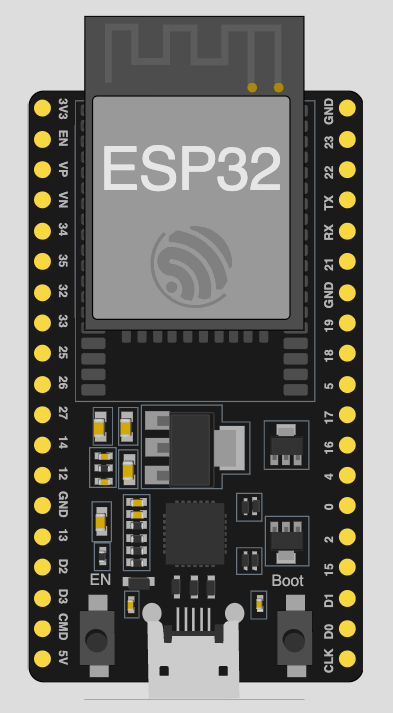
\includegraphics[width=0.8\linewidth]{esp32.png}
    \caption{Vi điều khiển ESP32}
    \label{fig:esp32}
  \end{minipage}\hfill
  \begin{minipage}{0.45\textwidth}
    \centering
    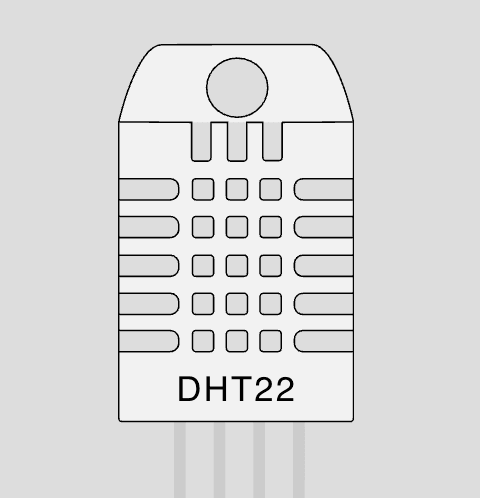
\includegraphics[width=0.8\linewidth]{dht22.png}
    \caption{Cảm biến DHT22}
    \label{fig:hw-dht22}
  \end{minipage}

  \vspace{0.5cm}

  \begin{minipage}{0.31\textwidth}
    \centering
    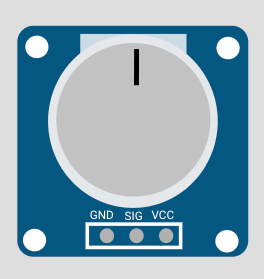
\includegraphics[width=0.8\linewidth]{potentiometer.png}
    \caption{Biến trở}
    \label{fig:hw-pot}
  \end{minipage}\hfill
  \begin{minipage}{0.31\textwidth}
    \centering
    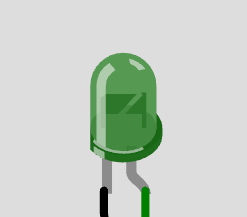
\includegraphics[width=0.8\linewidth]{led.png}
    \caption{Đèn LED}
    \label{fig:hw-led}
  \end{minipage}\hfill
  \begin{minipage}{0.31\textwidth}
    \centering
    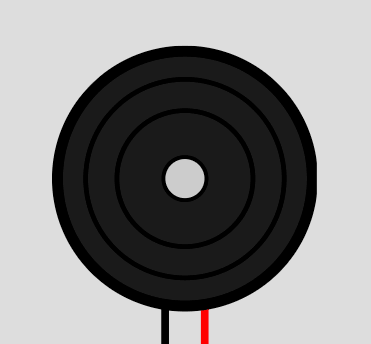
\includegraphics[width=0.8\linewidth]{buzzer.png}
    \caption{Còi Buzzer}
    \label{fig:hw-buzzer}
  \end{minipage}
\end{figure}

\subsection{Kết nối phần cứng (GPIO)}

Bảng~\ref{tbl:gpio} tóm tắt nối dây.

\begin{table}[H]
  \centering
  \caption{Bảng kết nối chân GPIO trên ESP32}
  \label{tbl:gpio}
  \begin{tabular}{|L{4cm}|C{4cm}|C{4.5cm}|}
    \hline
    \textbf{Chân ESP32} & \textbf{Nối đến} & \textbf{Chức năng} \\
    \hline
    3V3 & DHT22 VCC, Potentiometer VCC & Nguồn 3.3V cho cảm biến \\
    \hline
    GND & DHT22 GND, LED Cathode, Potentiometer GND, Buzzer GND & Chân nối đất chung \\
    \hline
    GPIO 4 & DHT22 DATA & Bus dữ liệu 1-wire (nhiệt độ + độ ẩm KK) \\
    \hline
    GPIO 5 & LED Anode (qua R220) & Điều khiển bật/tắt LED (mô phỏng bơm) \\
    \hline
    GPIO 18 & Buzzer (chân 2) & Phát âm thanh cảnh báo khi đất khô \\
    \hline
    GPIO 34 & Potentiometer SIG & Đọc giá trị độ ẩm đất (ADC, chỉ đọc) \\
    \hline
  \end{tabular}
\end{table}

\subsubsection{Sơ đồ logic (EasyEDA)}
Hình~\ref{fig:easyeda-schematic}.

\begin{figure}[H]
  \centering
  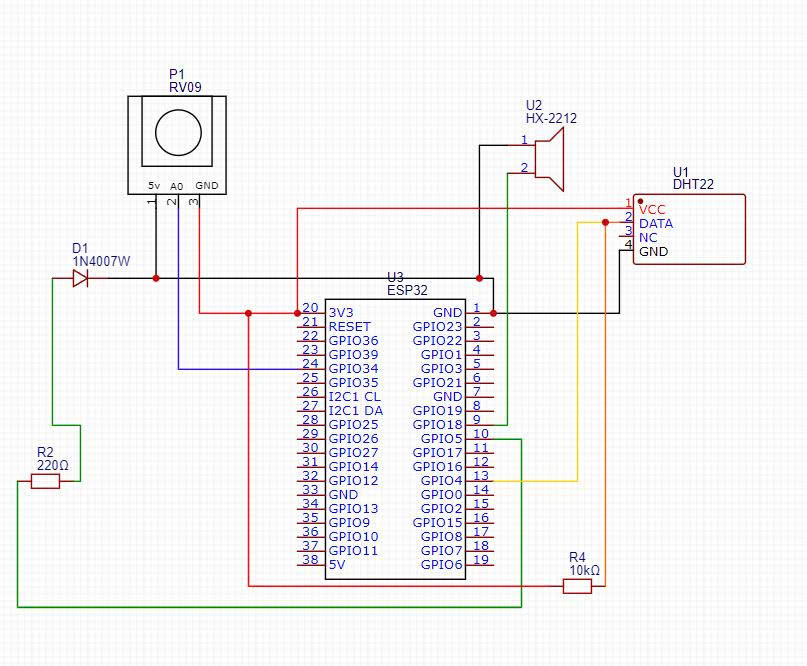
\includegraphics[width=0.95\linewidth]{mach-nguyen-ly-easyeda.png}
  \caption{Sơ đồ nguyên lý phần cứng (EasyEDA): ESP32, DHT22, đất, relay/bơm (mở rộng), buzzer, OLED (mở rộng) --- phần lõi đã code nằm ở DHT22, ADC đất, LED, buzzer}
  \label{fig:easyeda-schematic}
\end{figure}

\subsubsection{Mạch vật lý --- ảnh mô phỏng Wokwi (tương đương mạch thực tế đã nối)}
Hình~\ref{fig:wokwi}.

\begin{figure}[H]
  \centering
  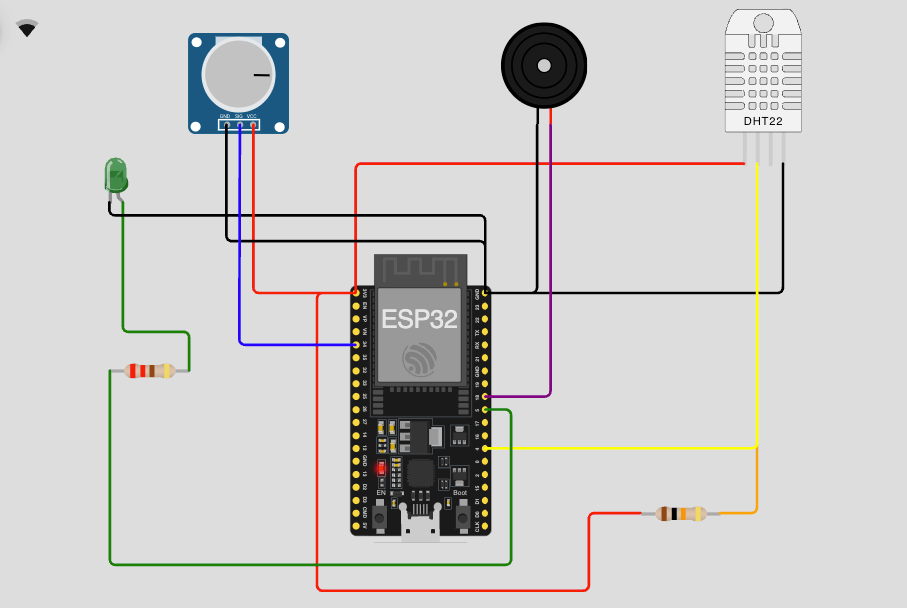
\includegraphics[width=0.88\linewidth]{mach-vat-ly-wokwi.png}
  \caption{Mạch mô phỏng Wokwi: ESP32 DevKit C v4 + DHT22 + LED + Potentiometer + Buzzer (khớp \file{diagram.json})}
  \label{fig:wokwi}
\end{figure}

\subsection{Giải thích các linh kiện chính}

\subsubsection{Vi điều khiển ESP32 DevKit C v4}
ESP32 là một hệ thống trên chip (SoC) tích hợp Wi-Fi và Bluetooth, được xây dựng trên nền vi xử lý Xtensa LX6 dual-core hiệu năng cao. Với bộ chuyển đổi tín hiệu tương tự sang số (ADC) 12-bit có độ phân giải cao, ESP32 có khả năng đọc chính xác các tín hiệu điện áp từ cảm biến analog. Trong hệ thống này, ESP32 đóng vai trò trung tâm điều phối: thu thập dữ liệu từ cảm biến, xử lý tín hiệu và duy trì kết nối liên tục lên đám mây qua giao thức MQTT bảo mật.

\begin{figure}[H]
  \centering
  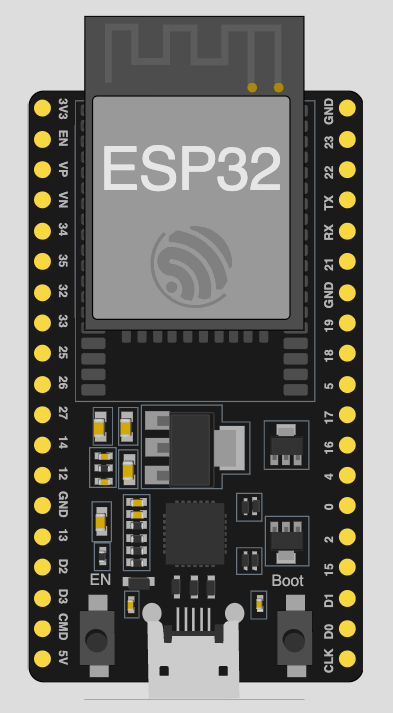
\includegraphics[width=0.42\linewidth]{esp32.png}
  \caption{Mạch vi điều khiển ESP32 DevKit C v4}
  \label{fig:hw_esp32_detail}
\end{figure}

\subsubsection{Cảm biến nhiệt độ và độ ẩm không khí DHT22}
DHT22 là cảm biến đo môi trường sử dụng giao tiếp số 1-wire, cho phép đo đồng thời nhiệt độ (độ chính xác $\pm$0.5\textdegree C) và độ ẩm không khí (độ chính xác $\pm$2--5\%). So với thế hệ trước (DHT11), DHT22 cải thiện đáng kể về phạm vi đo và độ phân giải, phù hợp cho các ứng dụng nông nghiệp yêu cầu theo dõi môi trường chính xác.

\begin{figure}[H]
  \centering
  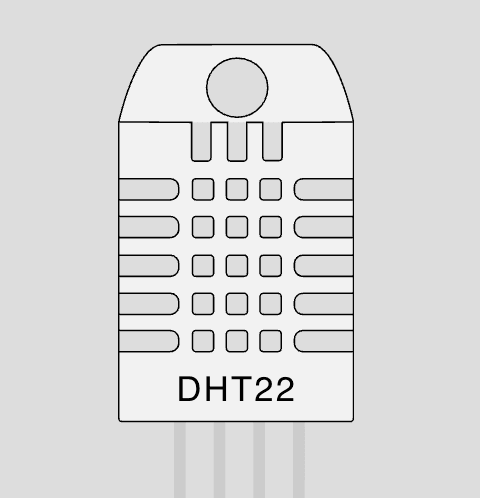
\includegraphics[width=0.38\linewidth]{dht22.png}
  \caption{Cảm biến DHT22 đo nhiệt độ và độ ẩm không khí}
  \label{fig:hw_dht22_detail}
\end{figure}

\subsubsection{Biến trở (mô phỏng cảm biến độ ẩm đất)}
Trong phạm vi mô phỏng của đề tài, biến trở (Potentiometer) được sử dụng thay thế cho cảm biến đo độ ẩm đất chuyên dụng. Khi xoay trục biến trở, điện trở thay đổi làm thay đổi mức điện áp trên chân tín hiệu, từ đó mô phỏng dải giá trị từ đất khô hoàn toàn đến đất bão hòa nước. Kết quả đọc được qua bộ ADC sẽ được quy đổi sang phần trăm độ ẩm để hiển thị trực quan trên Dashboard.

\begin{figure}[H]
  \centering
  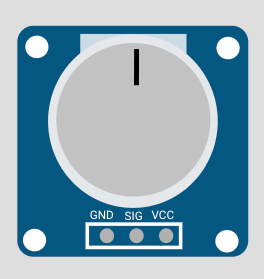
\includegraphics[width=0.38\linewidth]{potentiometer.png}
  \caption{Biến trở xoay dùng mô phỏng tín hiệu độ ẩm đất}
  \label{fig:hw_pot_detail}
\end{figure}

\subsubsection{Cơ cấu chấp hành và tín hiệu cảnh báo (LED \& Buzzer)}
Hệ thống sử dụng hai thiết bị đầu ra để phản ánh trực quan kết quả điều khiển. Đèn LED đóng vai trò giả lập trạng thái hoạt động của máy bơm nước: sáng khi bơm đang vận hành, tắt khi bơm ngừng. Còi sinh âm (Buzzer) được điều khiển bằng xung PWM, phát tín hiệu âm thanh cường độ cao khi hệ thống phát hiện độ ẩm đất xuống dưới ngưỡng cảnh báo khô hạn, nhằm thông báo kịp thời cho người vận hành.

\begin{figure}[H]
  \centering
  \begin{minipage}{0.46\textwidth}
    \centering
    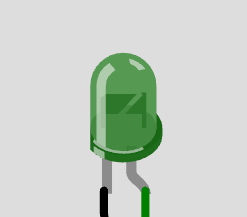
\includegraphics[width=0.65\linewidth]{led.png}
    \caption{Đèn LED mô phỏng trạng thái máy bơm}
    \label{fig:hw_led_detail}
  \end{minipage}\hfill
  \begin{minipage}{0.46\textwidth}
    \centering
    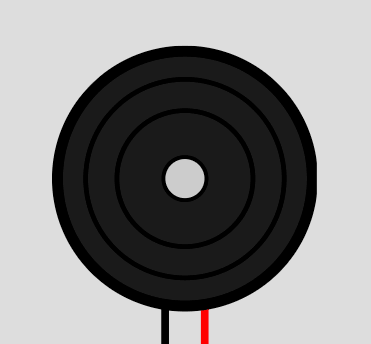
\includegraphics[width=0.65\linewidth]{buzzer.png}
    \caption{Còi Buzzer phát âm thanh cảnh báo}
    \label{fig:hw_buz_detail}
  \end{minipage}
\end{figure}


\subsection{Luồng hoạt động tóm tắt theo chức năng}

Toàn bộ hoạt động của hệ thống diễn ra theo một vòng lặp liên tục: vi điều khiển định kỳ thu thập dữ liệu từ các cảm biến, thực hiện kiểm tra ngưỡng để kích hoạt cảnh báo âm thanh khi cần, sau đó đóng gói kết quả thành bản tin JSON và gửi lên broker MQTT. Song song với đó, hệ thống luôn lắng nghe các lệnh điều khiển từ Dashboard để bật hoặc tắt máy bơm, đồng thời tự động ngắt bơm sau một khoảng thời gian chạy định sẵn nhằm tránh bơm hoạt động quá lâu. Chi tiết về sơ đồ kiến trúc và luồng dữ liệu được trình bày trong Chương~4.

\begin{figure}[H]
  \centering
  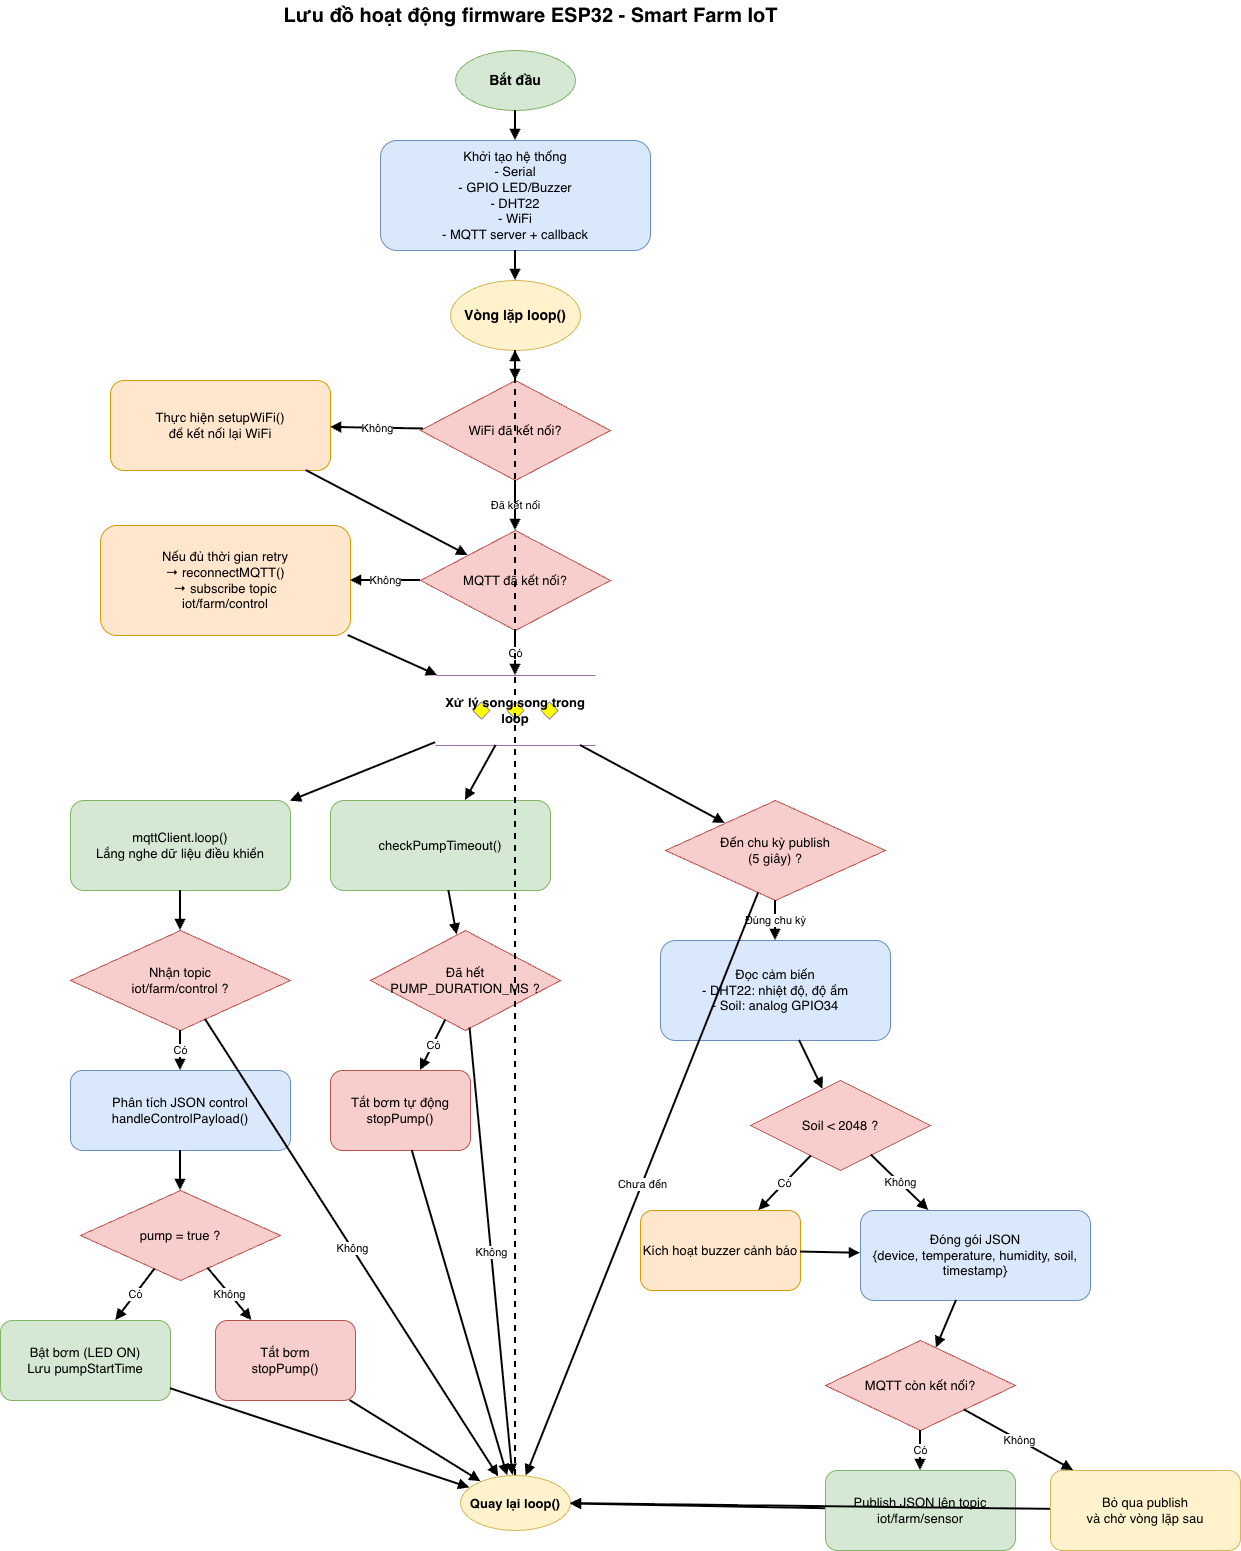
\includegraphics[width=0.92\linewidth]{image-3-4.png}
  \caption{Sơ đồ luồng hoạt động tóm tắt theo chức năng của hệ thống}
  \label{fig:luong-3-4}
\end{figure}


% =============================================================================
% 4. NGUYÊN LÝ HOẠT ĐỘNG
% =============================================================================
\section*{CHƯƠNG 4: NGUYÊN LÝ HOẠT ĐỘNG}
\phantomsection
\addcontentsline{toc}{section}{CHƯƠNG 4: NGUYÊN LÝ HOẠT ĐỘNG}
\label{sec:ch4}
\setcounter{section}{4}
\setcounter{subsection}{0}

\subsection{Sơ đồ luồng hệ thống (kiến trúc ba tầng)}

Kiến trúc của hệ thống được xây dựng dựa trên mô hình ba tầng tiêu chuẩn của một ứng dụng IoT hiện đại. Tầng dưới cùng là tầng thiết bị, bao gồm vi điều khiển ESP32 kết nối trực tiếp với các cảm biến và cơ cấu chấp hành. Tầng chính giữa là tầng trung gian, sử dụng dịch vụ Broker của HiveMQ Cloud với giao thức bảo mật TLS để chuyển tiếp dữ liệu một cách an toàn. Trên cùng là tầng ứng dụng với Node-RED Dashboard, đóng vai trò là giao diện trung tâm để người dùng giám sát các thông số môi trường và phát lệnh điều khiển ngược trở lại thiết bị qua các chủ đề (topic) đã được định nghĩa thống nhất.

\begin{figure}[H]
  \centering
  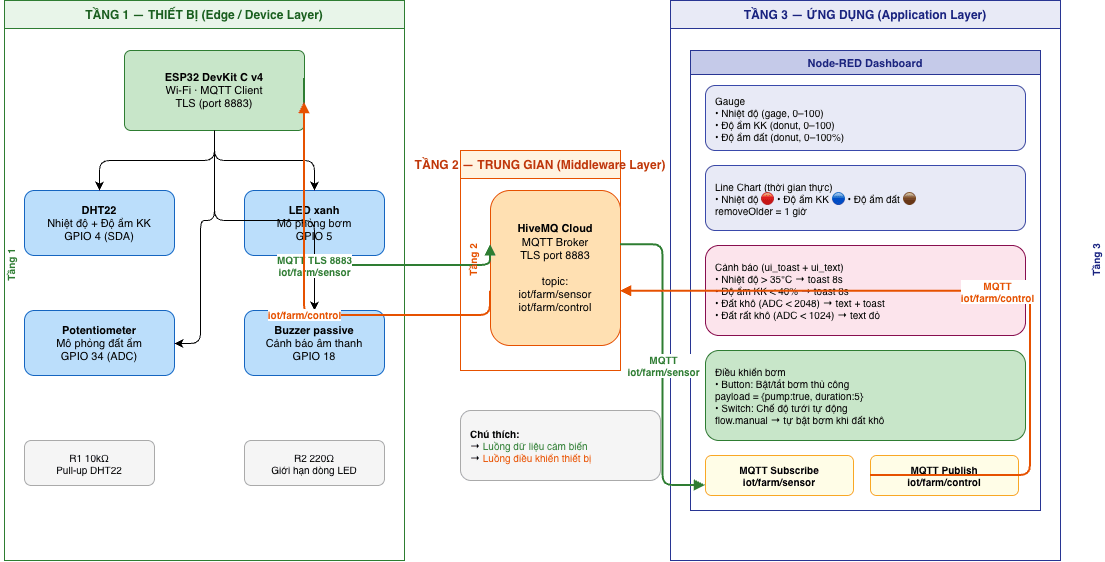
\includegraphics[width=0.88\linewidth]{so-do-kien-truc-he-thong.png}
  \caption{Sơ đồ kiến trúc tổng thể hệ thống giám sát và điều khiển môi trường trang trại thông minh}
  \label{fig:kien-truc}
\end{figure}

\subsection{Luồng giám sát: cảm biến $\rightarrow$ MQTT $\rightarrow$ Dashboard}

Luồng giám sát được thực hiện theo cơ chế định kỳ: cứ mỗi chu kỳ 5 giây, vi điều khiển đọc dữ liệu từ cảm biến nhiệt độ, độ ẩm không khí và tín hiệu ADC từ biến trở mô phỏng độ ẩm đất. Toàn bộ dữ liệu được đóng gói thành một bản tin JSON có cấu trúc thống nhất rồi gửi lên MQTT Broker (HiveMQ Cloud) qua kết nối bảo mật TLS. Broker sau đó phân phát bản tin tới Node-RED — nơi các luồng xử lý song song phân tích giá trị và cập nhật lên các widget tương ứng trên Dashboard: đồng hồ đo (gauge), biểu đồ theo thời gian thực (line chart) và thông báo cảnh báo (toast notification). Kiến trúc ba tầng của luồng này được minh họa tại Hình~\ref{fig:kien-truc} (mục~4.1).


\subsection{Luồng điều khiển: Dashboard $\rightarrow$ MQTT $\rightarrow$ ESP32 (LED mô phỏng bơm)}

Người dùng bấm nút hoặc kích hoạt tưới tự động trên Dashboard; Node-RED publish JSON xuống \code{iot/farm/control}; \code{mqttCallback()} $\rightarrow$ \code{handleControlPayload()} bật LED và ghi \code{pumpStartTime}.

ESP32 thực hiện chu trình: khởi tạo Serial 115200, Wi-Fi, DHT, GPIO, MQTT TLS, subscribe \code{iot/farm/control}. Vòng \code{loop()}: duy trì Wi-Fi/MQTT, \code{checkPumpTimeout()}, mỗi 5\,s đọc cảm biến, buzzer nếu đất khô, \code{publishSensorData()} nếu broker sẵn sàng.

\begin{figure}[H]
  \centering
  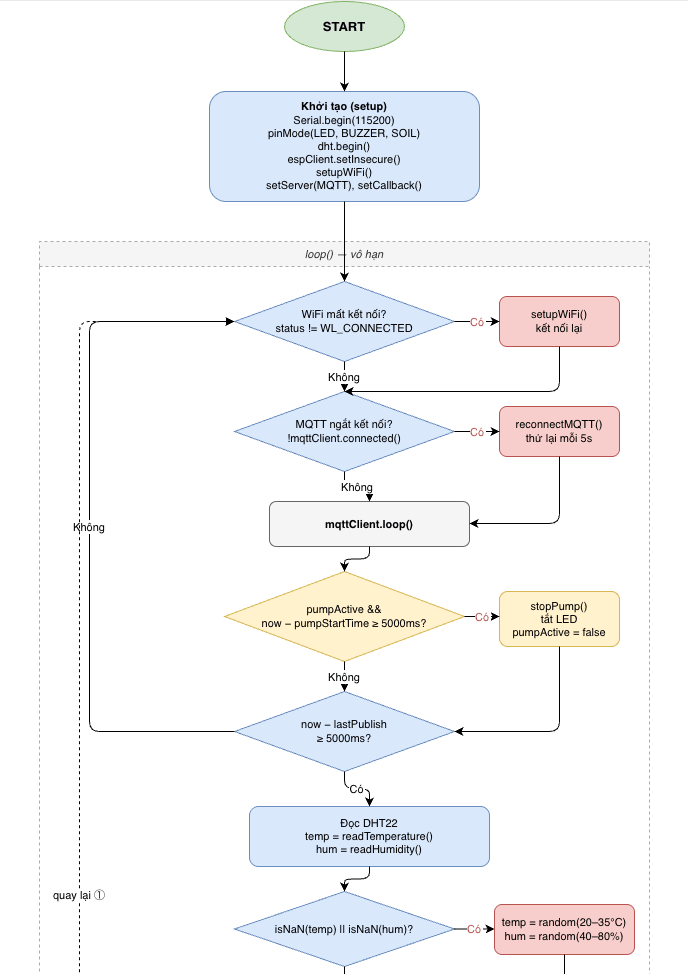
\includegraphics[width=0.88\linewidth]{luu-do-thuat-toan-top.png}
  \caption{Lưu đồ thuật toán trên ESP32 (phần trên: \code{setup()}, \code{loop()} --- Wi-Fi, MQTT, timeout bơm, nhịp 5 giây)}
  \label{fig:luudo}
\end{figure}

\begin{figure}[H]
  \centering
  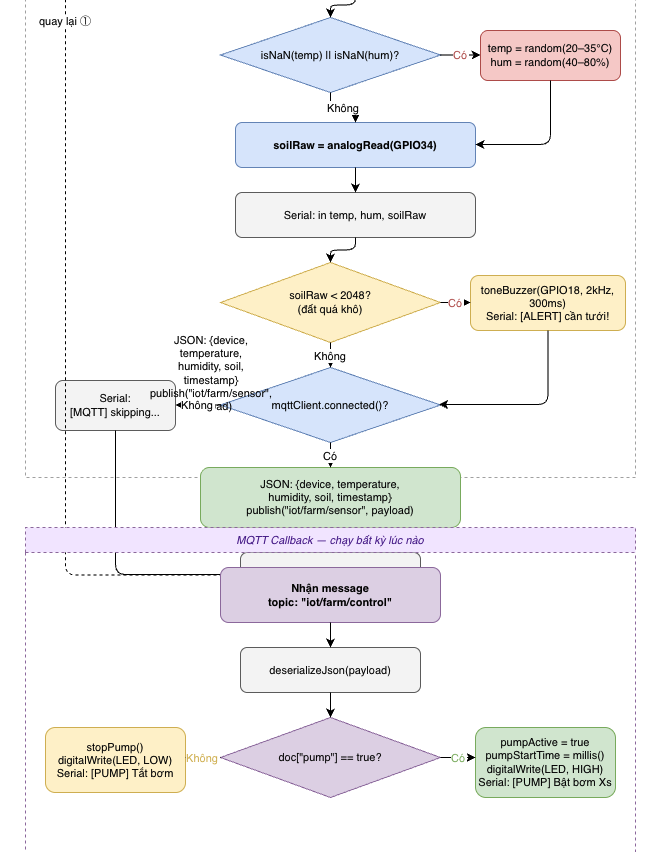
\includegraphics[width=0.88\linewidth]{luu-do-thuat-toan-bottom.png}
  \caption{Lưu đồ thuật toán trên ESP32 (phần dưới: đọc cảm biến, buzzer, publish và \code{mqttCallback} nhận \code{iot/farm/control})}
  \label{fig:luudo-2}
\end{figure}

\subsection{Luồng đồng bộ trạng thái bơm và giới hạn thời gian chạy}

Để tránh tình trạng máy bơm hoạt động không kiểm soát, hệ thống triển khai cơ chế giám sát thời gian chạy tự động. Ngay khi nhận lệnh kích hoạt bơm từ Dashboard, vi điều khiển ghi lại thời điểm bắt đầu và theo dõi thời gian đã trôi qua. Khi thời gian vận hành đạt ngưỡng giới hạn định sẵn (5 giây), hệ thống tự động ngắt bơm và cập nhật trạng thái đèn LED tương ứng — đảm bảo hành vi thực tế của thiết bị luôn đồng bộ với trạng thái hiển thị trên giao diện điều khiển.

\subsection{Luồng tưới tự động theo ngưỡng độ ẩm đất (Node-RED)}

Chế độ tưới tự động được kích hoạt dựa trên hai điều kiện đồng thời: giá trị độ ẩm đất đo được thấp hơn ngưỡng cảnh báo khô hạn, và người dùng đã bật chế độ tự động trên Dashboard. Khi cả hai điều kiện này được thỏa mãn, Node-RED tự động phát lệnh kích hoạt bơm mà không cần can thiệp thủ công. Cơ chế này hoàn toàn dựa trên giá trị cảm biến thực tế, không phụ thuộc vào lịch thời gian hay đồng hồ hệ thống.

\subsection{Luồng duy trì kết nối Wi-Fi và MQTT}

Tính ổn định của hệ thống IoT phụ thuộc lớn vào khả năng tự phục hồi kết nối mạng. Vi điều khiển liên tục kiểm tra trạng thái kết nối Wi-Fi trong mỗi vòng lặp; nếu phát hiện mất kết nối, hệ thống tự động thực hiện kết nối lại mà không làm gián đoạn các tác vụ khác. Tương tự, nếu phiên kết nối MQTT bị ngắt, hệ thống định kỳ thử kết nối lại tối đa mỗi 5 giây — đảm bảo luồng dữ liệu cảm biến và các lệnh điều khiển không bị gián đoạn lâu dài.


% =============================================================================
% 5. CÀI ĐẶT HỆ THỐNG
% =============================================================================
\section*{CHƯƠNG 5: CÀI ĐẶT HỆ THỐNG}
\phantomsection
\addcontentsline{toc}{section}{CHƯƠNG 5: CÀI ĐẶT HỆ THỐNG}
\label{sec:ch5}
\setcounter{section}{5}
\setcounter{subsection}{0}

\subsection{Chuẩn bị công cụ và môi trường phát triển}

Trước khi tiến hành cài đặt, người dùng cần chuẩn bị các phần mềm và môi trường nền tảng sau để đảm bảo hệ thống vận hành ổn định:
\begin{itemize}
    \item \textbf{Visual Studio Code:} Trình soạn thảo mã nguồn chính, tải tại \url{https://code.visualstudio.com/}.
    \item \textbf{PlatformIO IDE:} Tiện ích mở rộng trong VS Code dùng để quản lý dư án và thư viện cho ESP32, thông tin tại \url{https://platformio.org/}.
    \item \textbf{Node.js:} Nền tảng thực thi JavaScript phía máy chủ, tải phiên bản LTS tại \url{https://nodejs.org/}.
    \item \textbf{Node-RED:} Công cụ lập trình luồng (flow-based), hướng dẫn cài đặt tại \url{https://nodered.org/docs/getting-started/local}.
\end{itemize}

\subsection{Khởi tạo sơ đồ mạch mô phỏng và cấu hình phần cứng}

Trong đề tài này, việc kiểm thử phần cứng được thực hiện thông qua nền tảng mô phỏng trực tuyến Wokwi (\url{https://wokwi.com/}). Quy trình thiết lập như sau:
\begin{enumerate}
    \item Truy cập Wokwi và khởi tạo một dự án ESP32 mới.
    \item Sao chép toàn bộ nội dung mã nguồn JSON tại \textbf{Phụ lục C (Sơ đồ mạch Wokwi)}.
    \item Mở thẻ \file{diagram.json} trong trình soạn thảo của Wokwi và dán nội dung đã sao chép vào.
    \item Hệ thống sẽ tự động khởi tạo các linh kiện (ESP32, DHT22, Biến trở, LED, Buzzer) và các kết nối dây tương ứng theo đúng thiết kế của đề tài.
\end{enumerate}

\subsection{Triển khai và vận hành Firmware cho ESP32}

\subsubsection{Cài đặt mã nguồn và thư viện}
Người dùng thực hiện sao chép toàn bộ mã nguồn chương trình tại \textbf{Phụ lục A (Mã nguồn ESP32)} và dán vào tệp \file{main.cpp} trong dự án PlatformIO hoặc thẻ \file{sketch.ino} trên Wokwi. Các thư viện như \textit{DHT sensor library}, \textit{PubSubClient} và \textit{ArduinoJson} sẽ được hệ thống tự động nhận diện và quản lý.

\subsubsection{Cấu hình thông số hệ thống}
Để thiết bị có thể kết nối với hạ tầng đám mây, cần cập nhật các thông số sau trong tệp mã nguồn:
\begin{itemize}
    \item \textbf{Kết nối mạng:} Cập nhật tên và mật khẩu Wi-Fi. (Trên Wokwi mặc định dùng tên dự án và mật khẩu trống hoặc mạng giả lập).
    \item \textbf{Xác thực MQTT:} Cập nhật các thông tin định danh bao gồm địa chỉ máy chủ, tên đăng nhập và mật khẩu truy cập (Broker, Username, Password) sao cho khớp với tài khoản HiveMQ Cloud đã đăng ký.
\end{itemize}

\subsubsection{Vận hành mô phỏng}
Vì hệ thống sử dụng môi trường mô phỏng Wokwi, người dùng không cần kết nối thiết bị vật lý qua cổng USB. Chỉ cần nhấn nút \textbf{Start Simulation} để bắt đầu chạy chương trình. Toàn bộ quá trình kết nối và dữ liệu cảm biến sẽ được hiển thị trực tiếp qua cửa sổ \textit{Serial Monitor} của trình giả lập.

\subsection{Thiết lập hệ thống điều khiển và giao diện Node-RED}

\subsubsection{Lệnh cài đặt nền tảng}
Mở cửa sổ dòng lệnh (Terminal) và thực hiện cài đặt Node-RED cùng giao diện Dashboard thông qua trình quản lý gói npm:
\begin{lstlisting}[language=bash, basicstyle=\ttfamily\small, frame=none, numbers=none]
npm install -g node-red
npm install -g node-red-dashboard
\end{lstlisting}
Sau đó, gõ lệnh \code{node-red} để khởi động dịch vụ và truy cập vào địa trị \url{http://127.0.0.1:1880}.

\subsubsection{Triển khai luồng xử lý và giao diện Dashboard}
Để thiết lập logic điều khiển và giao diện, người dùng thực hiện:
\begin{enumerate}
    \item Sao chép mã nguồn JSON tại \textbf{Phụ lục B (Mã nguồn Node-RED Flow)}.
    \item Tại giao diện Node-RED, chọn \textbf{Menu} $\rightarrow$ \textbf{Import} và dán nội dung vào cửa sổ hiện ra.
    \item Nhấn \textbf{Import} để hệ thống tự động tạo ra các luồng xử lý và giao diện Dashboard.
    \item Cập nhật cấu hình node \textbf{mqtt-broker} để thiết lập thông tin đăng nhập HiveMQ Cloud tương tự như phía ESP32.
\end{enumerate}

\subsection{Vận hành và kiểm thử tổng thể}
Sau khi hoàn tất cài đặt, người dùng truy cập Dashboard tại \url{http://127.0.0.1:1880/ui}. Hệ thống hoạt động đúng khi các đồng hồ đo hiển thị giá trị nhiệt độ, độ ẩm thực tế từ Wokwi, và người dùng có thể thực hiện bật/tắt máy bơm từ xa thông qua các nút nhấn trên giao diện.

\begin{figure}[H]
  \centering
  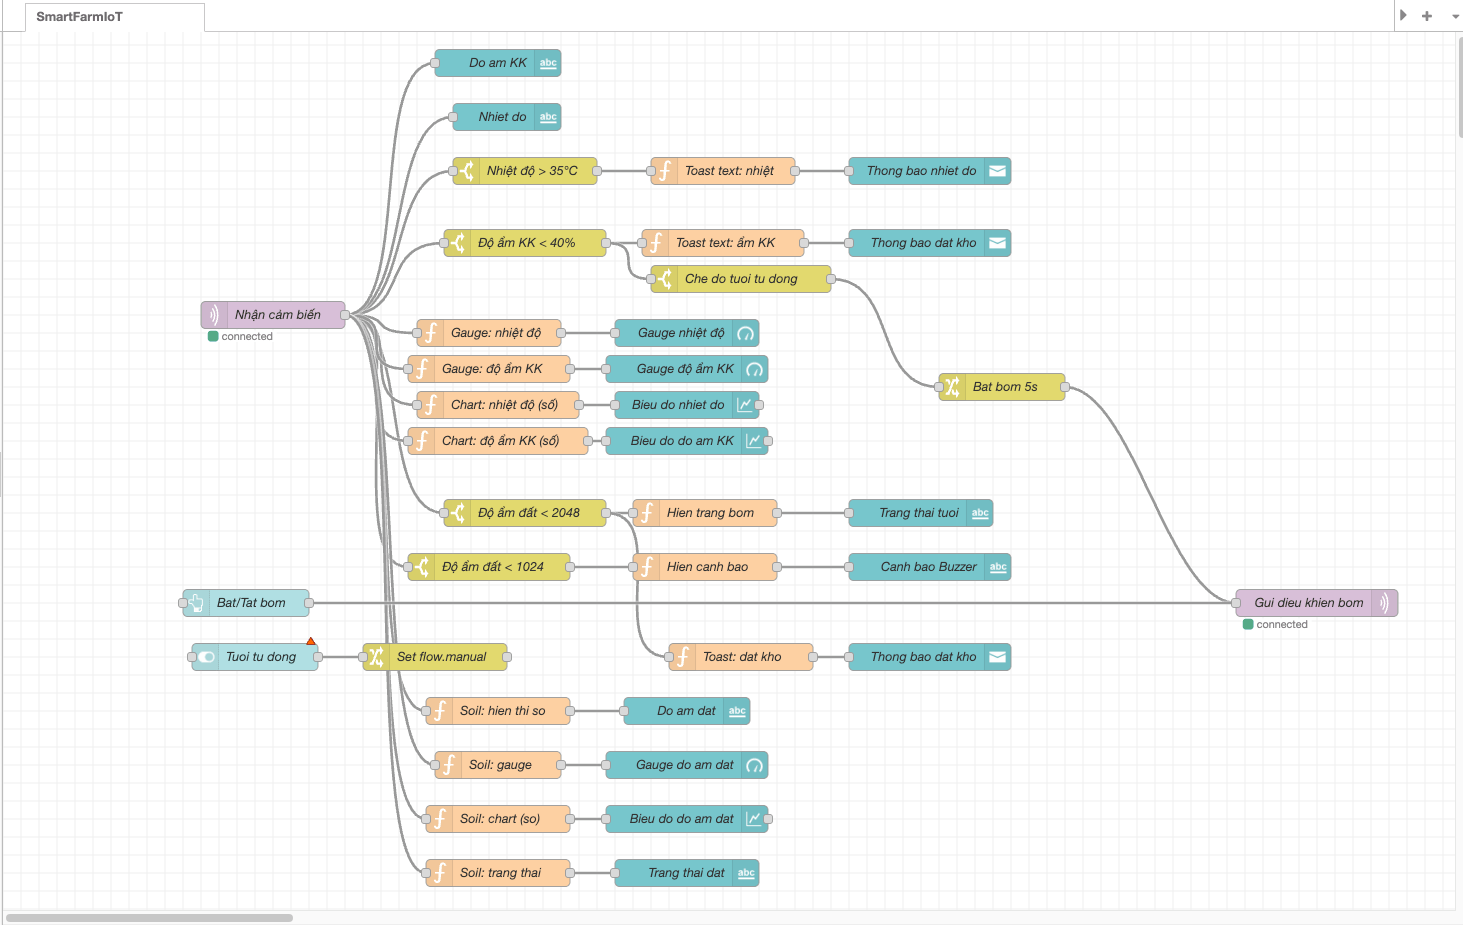
\includegraphics[width=0.9\linewidth]{nodered-flow-full.png}
  \caption{Giao diện editor Node-RED với flow đầy đủ}
  \label{fig:nr-flow}
\end{figure}

\begin{figure}[H]
  \centering
  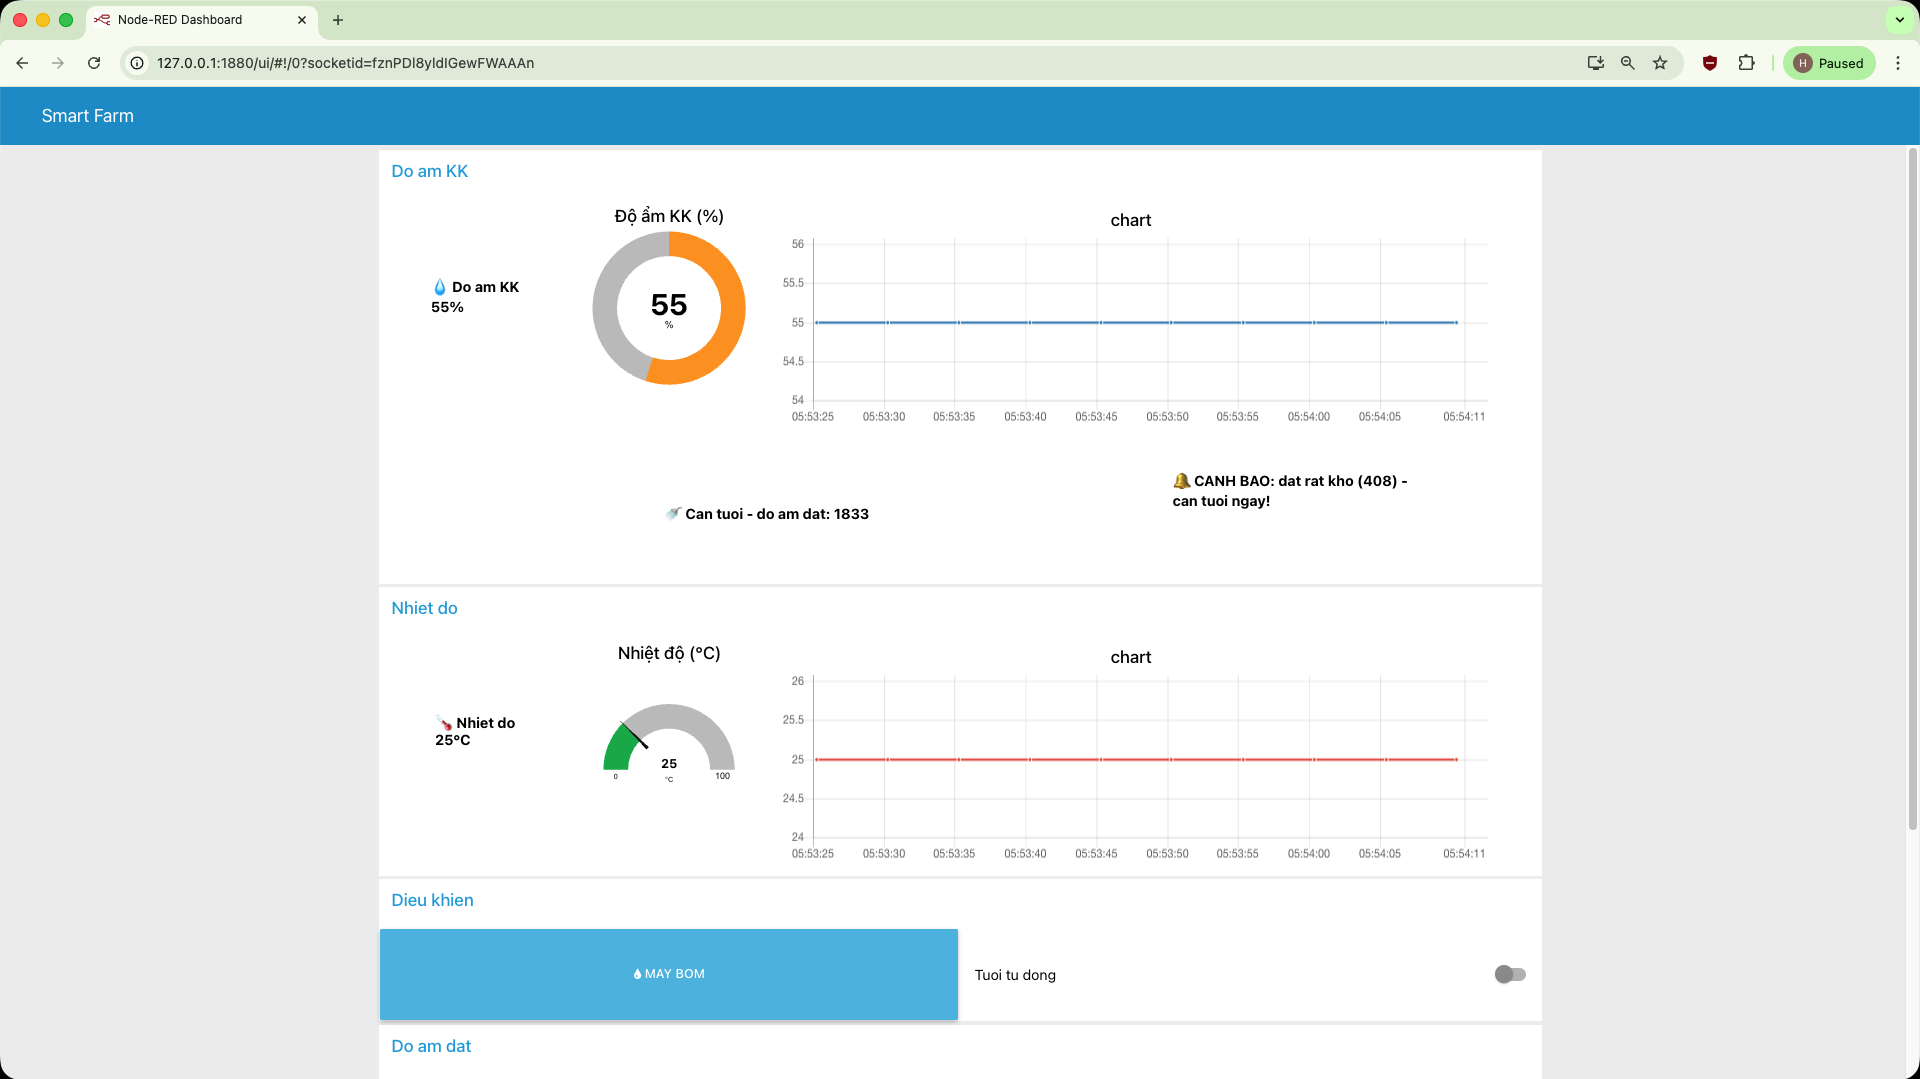
\includegraphics[width=0.9\linewidth]{nodered-dashboard-full-1.png}
  \caption{Giao diện Dashboard Node-RED (phần 1/2): độ ẩm không khí, nhiệt độ, điều khiển máy bơm và tưới tự động, phần đầu nhóm độ ẩm đất}
  \label{fig:nr-dash-1}
\end{figure}

\begin{figure}[H]
  \centering
  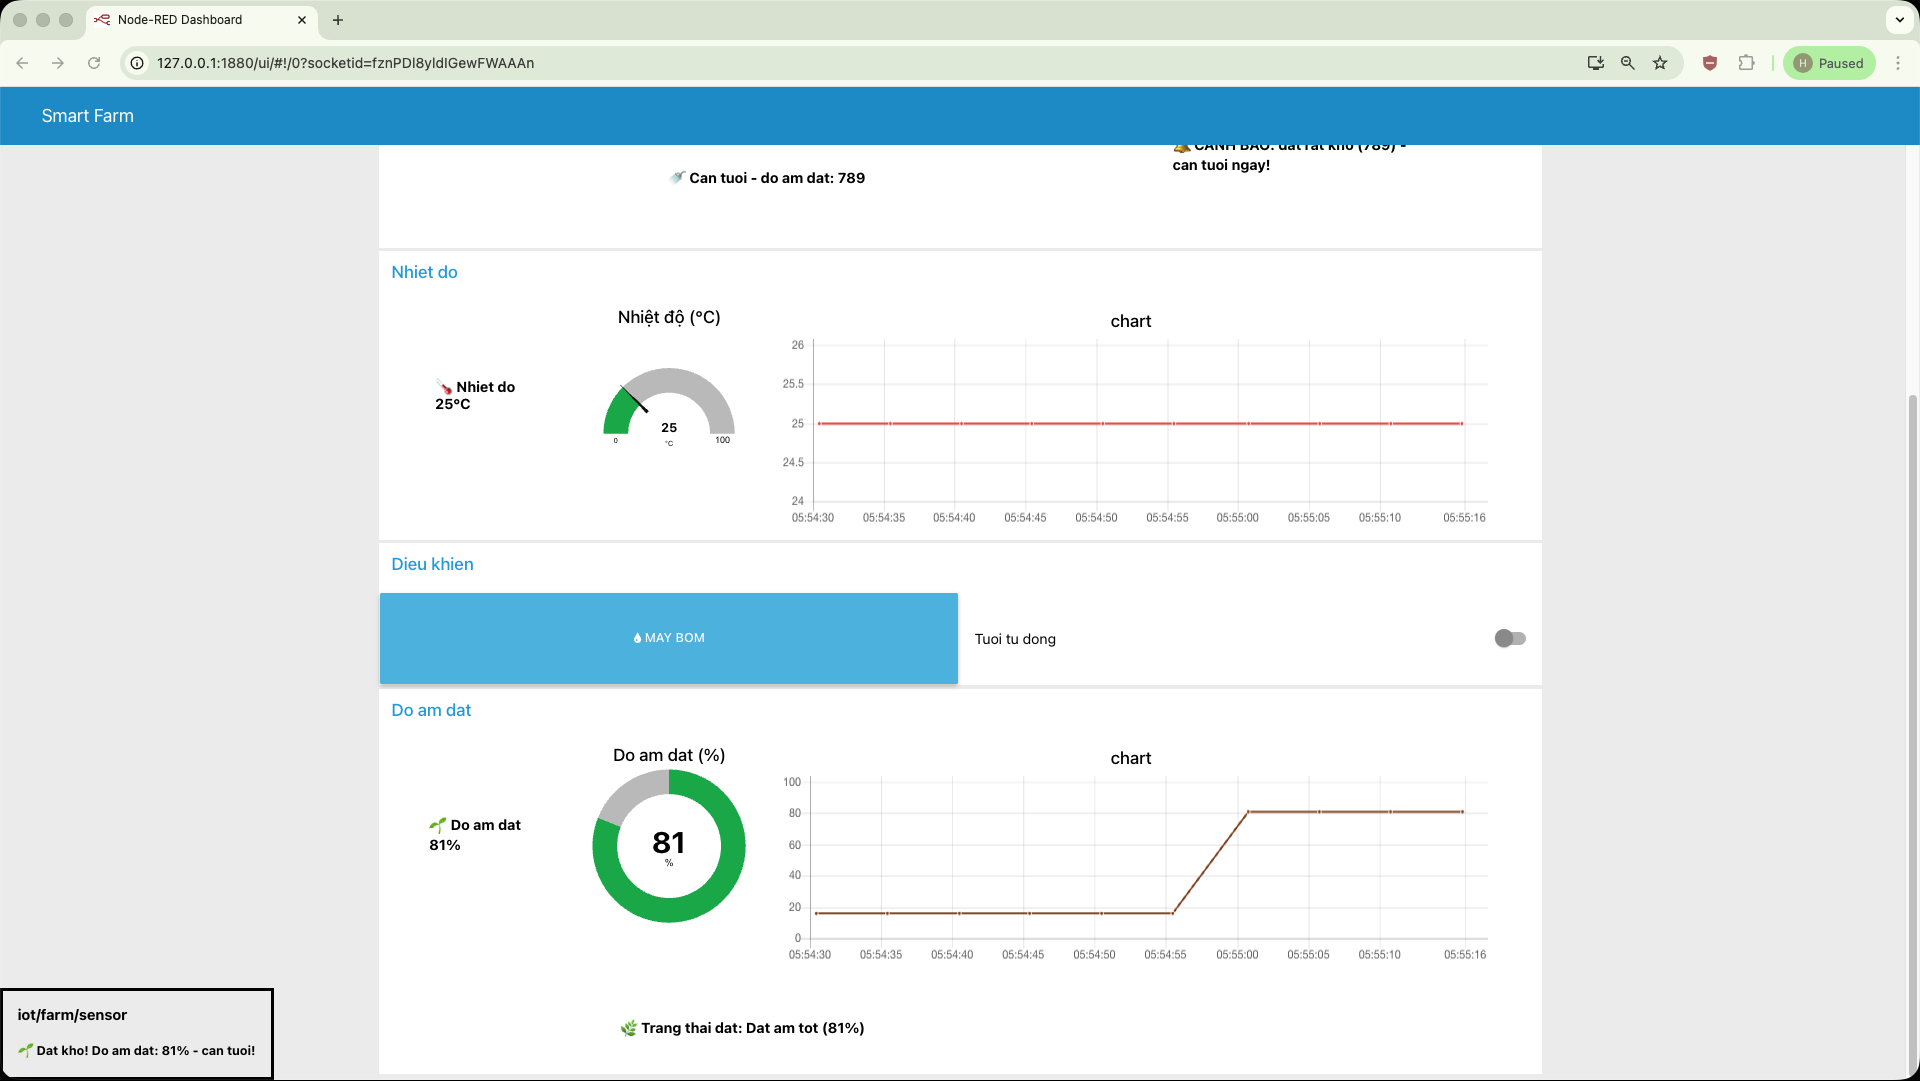
\includegraphics[width=0.9\linewidth]{nodered-dashboard-full-2.png}
  \caption{Giao diện Dashboard Node-RED (phần 2/2): nhiệt độ, điều khiển, độ ẩm đất (gauge, biểu đồ line, trạng thái đất và cảnh báo)}
  \label{fig:nr-dash-2}
\end{figure}

% =============================================================================
% 6. KẾT QUẢ THỰC HIỆN
% =============================================================================
\section*{CHƯƠNG 6: KẾT QUẢ THỰC HIỆN}
\phantomsection
\addcontentsline{toc}{section}{CHƯƠNG 6: KẾT QUẢ THỰC HIỆN}
\label{sec:ch6}
\setcounter{section}{6}
\setcounter{subsection}{0}

\subsection{Kết quả mô phỏng phần cứng trên Wokwi}
Mạch điện của hệ thống được thực hiện mô phỏng đầy đủ trên nền tảng Wokwi. Hình~\ref{fig:res-wokwi} cho thấy sự kết nối chính xác giữa ESP32 và các linh kiện như cảm biến DHT22, biến trở mô phỏng độ ẩm đất, còi báo động Buzzer và đèn LED giả lập máy bơm.

\begin{figure}[H]
  \centering
  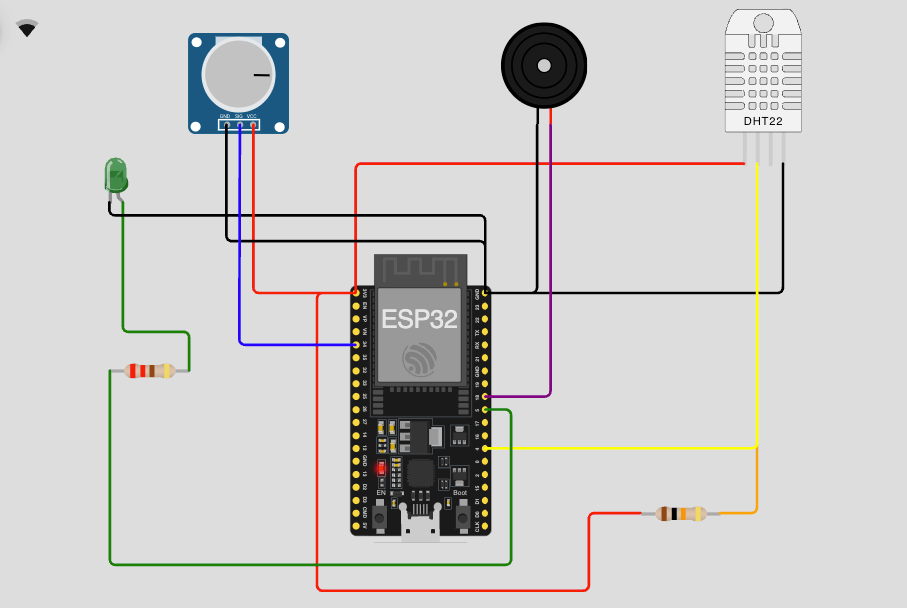
\includegraphics[width=0.88\linewidth]{mach-vat-ly-wokwi.png}
  \caption{Mô phỏng sơ đồ kết nối phần cứng thực tế trên môi trường Wokwi}
  \label{fig:res-wokwi}
\end{figure}

\subsection{Kết quả truyền nhận dữ liệu qua Serial Monitor}
Trong quá trình vận hành, vi điều khiển ESP32 liên tục gửi các thông tin trạng thái hoạt động lên cửa sổ Serial Monitor. Các thông tin bao gồm quá trình kết nối Wi-Fi, trạng thái thiết lập kết nối bảo mật TLS với HiveMQ Cloud và dữ liệu cảm biến thu thập được trước khi đóng gói JSON (Hình~\ref{fig:res-serial}).

\begin{figure}[H]
  \centering
  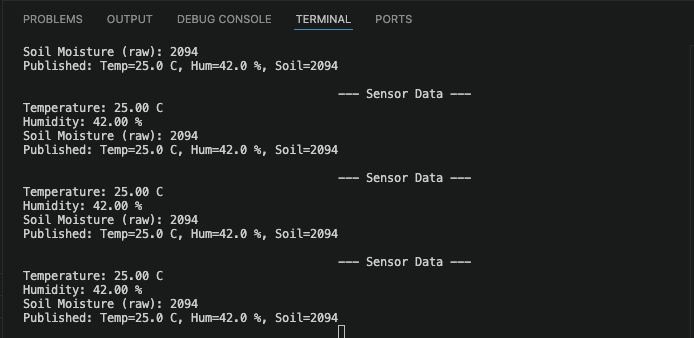
\includegraphics[width=0.85\linewidth]{serial-monitor.png}
  \caption{Dữ liệu log hoạt động và trạng thái kết nối MQTT trên Serial Monitor}
  \label{fig:res-serial}
\end{figure}

\subsection{Thiết lập luồng xử lý dữ liệu trên Node-RED}
Mọi chương trình xử lý phía máy chủ được tổ chức thành các luồng (flow) trực quan trên Node-RED. Hình~\ref{fig:res-nr-flow} thể hiện toàn bộ các node chức năng từ việc tiếp nhận dữ liệu MQTT, giải mã JSON đến việc phân luồng hiển thị và logic điều khiển máy bơm tự động.

\begin{figure}[H]
  \centering
  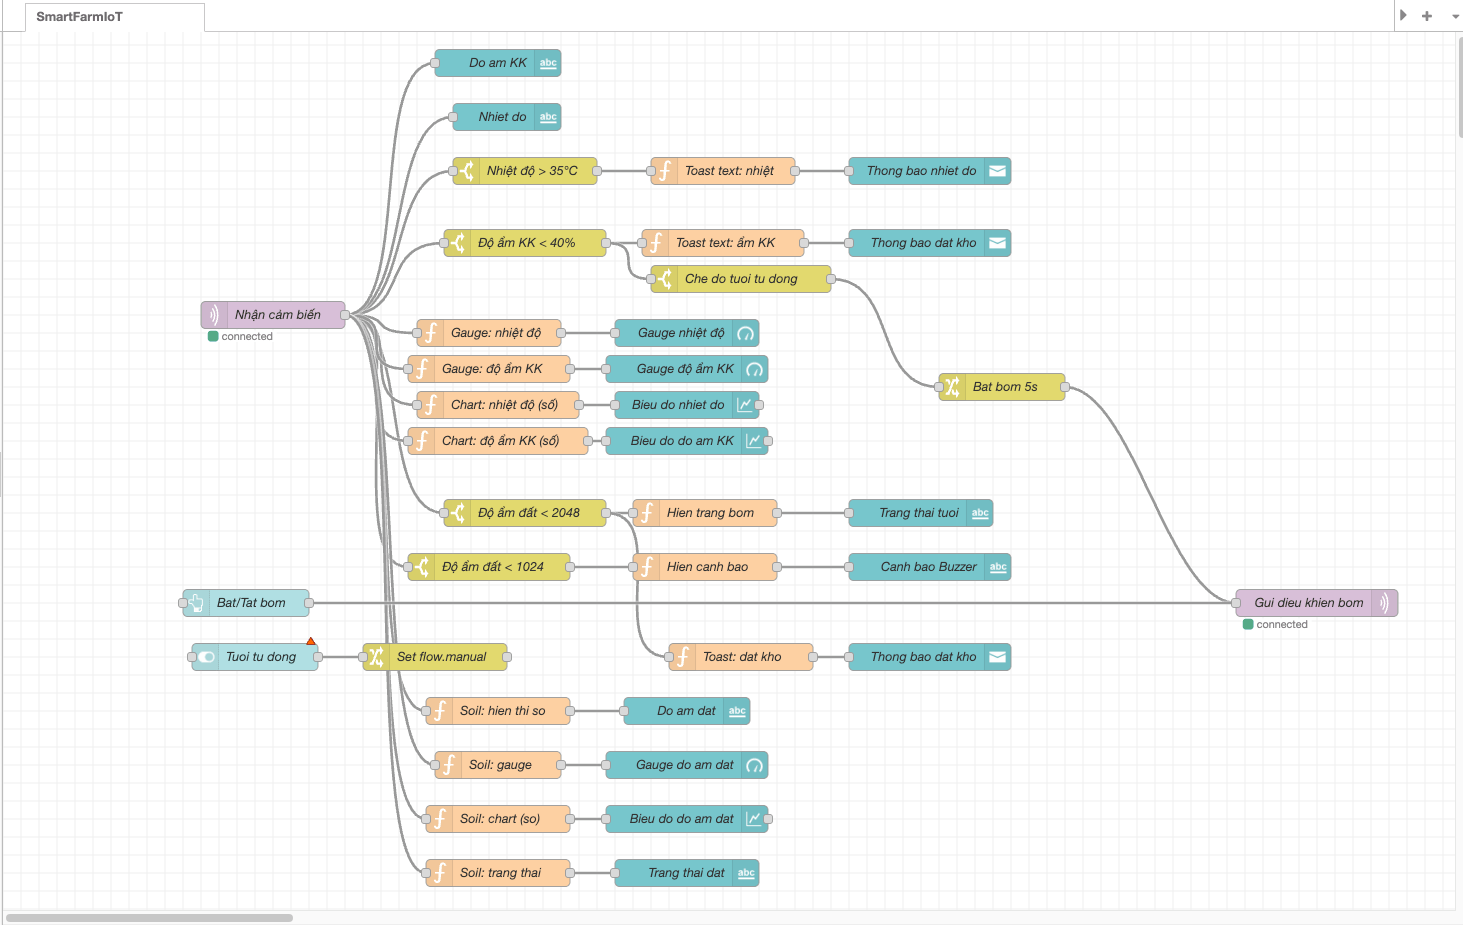
\includegraphics[width=0.92\linewidth]{nodered-flow-full.png}
  \caption{Sơ đồ luồng xử lý dữ liệu (Flow) đầy đủ trên trình biên tập Node-RED}
  \label{fig:res-nr-flow}
\end{figure}

\subsection{Giao diện giám sát và điều khiển Dashboard}
Kết quả quan trọng nhất của hệ thống là giao diện tương tác người dùng hiện đại và trực quan. Hệ thống Dashboard cung cấp đầy đủ các thông tin cần thiết về môi trường trang trại theo thời gian thực (Hình~\ref{fig:res-dash-1} và Hình~\ref{fig:res-dash-2}).

\begin{figure}[H]
  \centering
  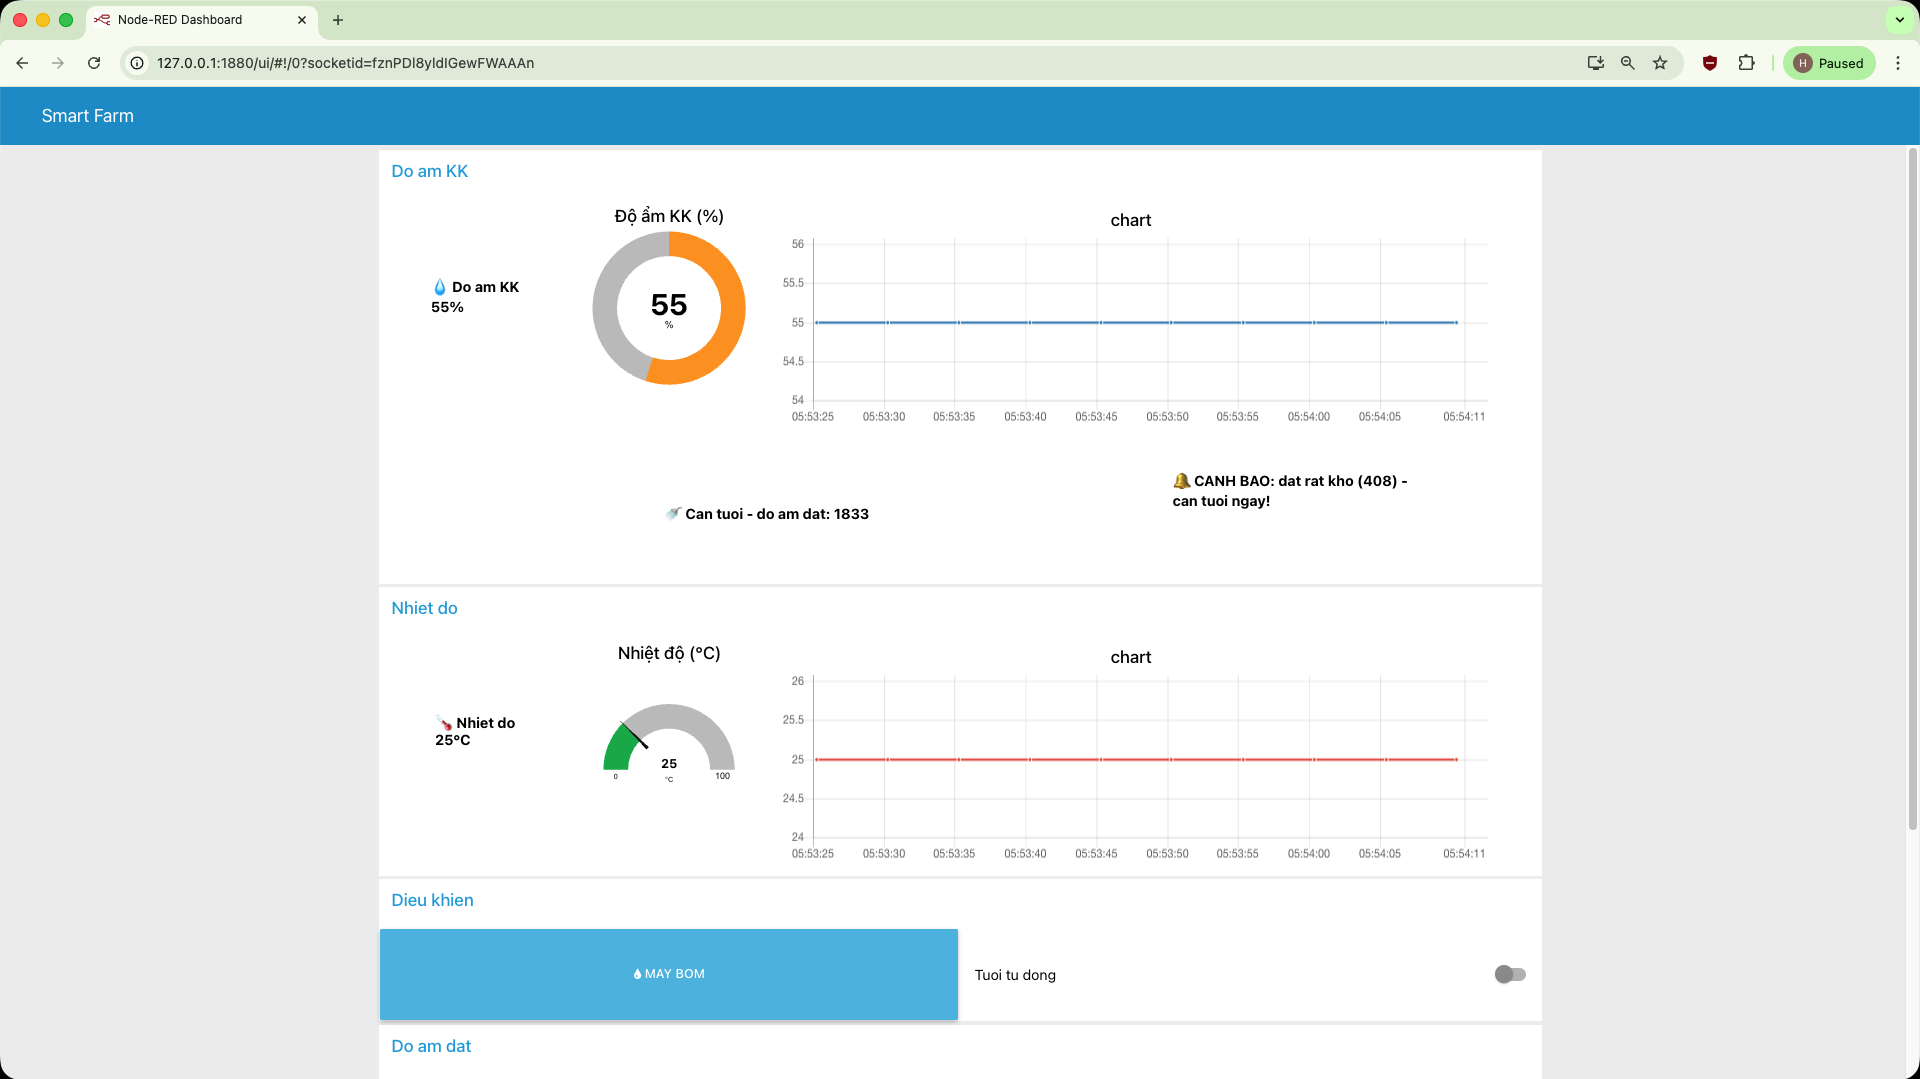
\includegraphics[width=0.9\linewidth]{nodered-dashboard-full-1.png}
  \caption{Giao diện Dashboard (Phần 1): Hiển thị đồng hồ đo và các nút điều khiển trung tâm}
  \label{fig:res-dash-1}
\end{figure}

\begin{figure}[H]
  \centering
  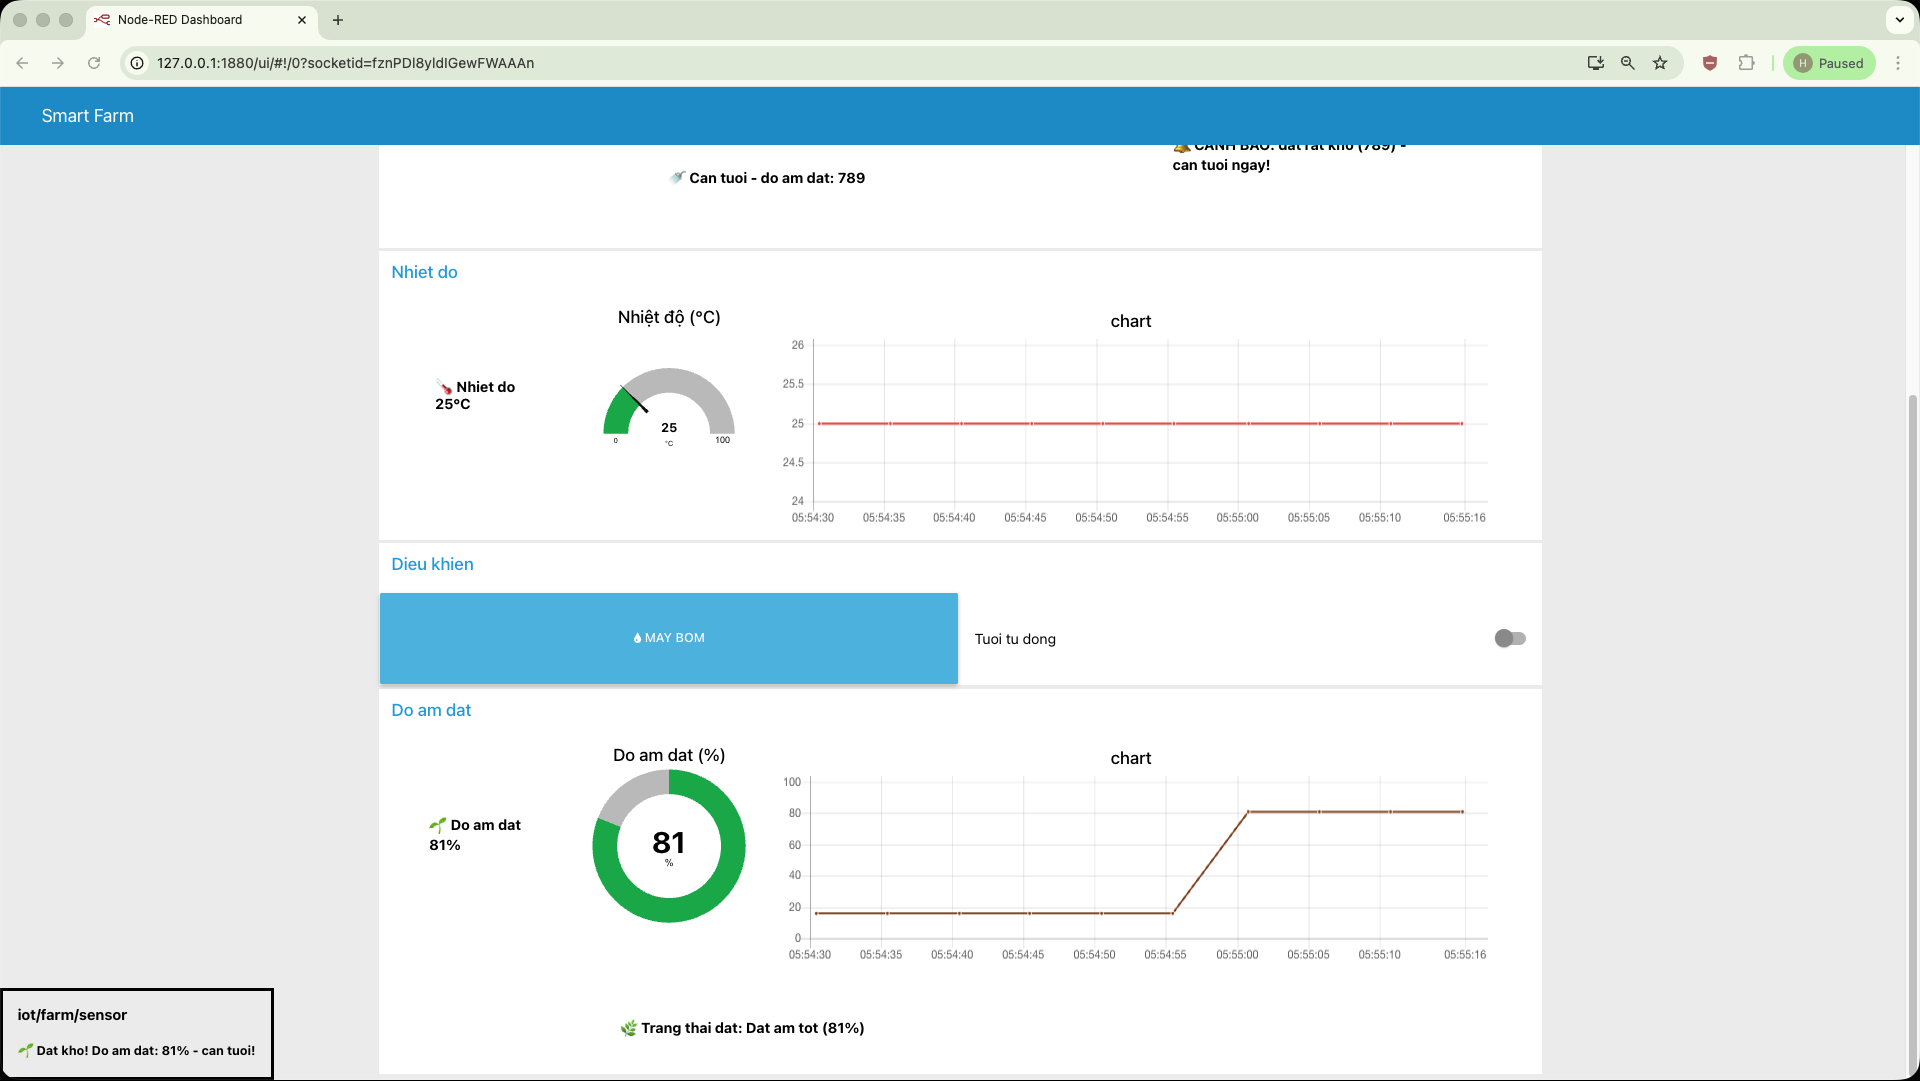
\includegraphics[width=0.9\linewidth]{nodered-dashboard-full-2.png}
  \caption{Giao diện Dashboard (Phần 2): Biểu đồ lịch sử dữ liệu và các thông tin trạng thái đất}
  \label{fig:res-dash-2}
\end{figure}

\subsection{Phân tích luồng hoạt động thực tế}

Hệ thống được thiết kế để xử lý các tình huống môi trường thực tế thông qua các cơ chế phản hồi tự động và cảnh báo trực quan (Hình~\ref{fig:res-alerts}).

\textbf{Cơ chế cảnh báo:} Khi các thông số vượt ngưỡng an toàn, hệ thống sẽ tự động kích hoạt các chỉ báo:
\begin{itemize}
    \item \textbf{Nhiệt độ:} Khi nhiệt độ $>$ 35$^\circ$C, Dashboard hiển thị toast cảnh báo nhiệt độ cao.
    \item \textbf{Độ ẩm không khí:} Khi độ ẩm $<$ 40\%, hệ thống gợi ý thực hiện tưới nước thông qua thông báo.
    \item \textbf{Độ ẩm đất:} Khi mức ADC $<$ 2048, toast cảnh báo đất khô sẽ xuất hiện và còi Buzzer trên ESP32 phát âm thanh báo động. Đặc biệt, khi độ ẩm giảm sâu (ADC $<$ 1024), Dashboard sẽ hiển thị cảnh báo mức đỏ cực kỳ khô hạn.
\end{itemize}

\begin{figure}[H]
  \centering
  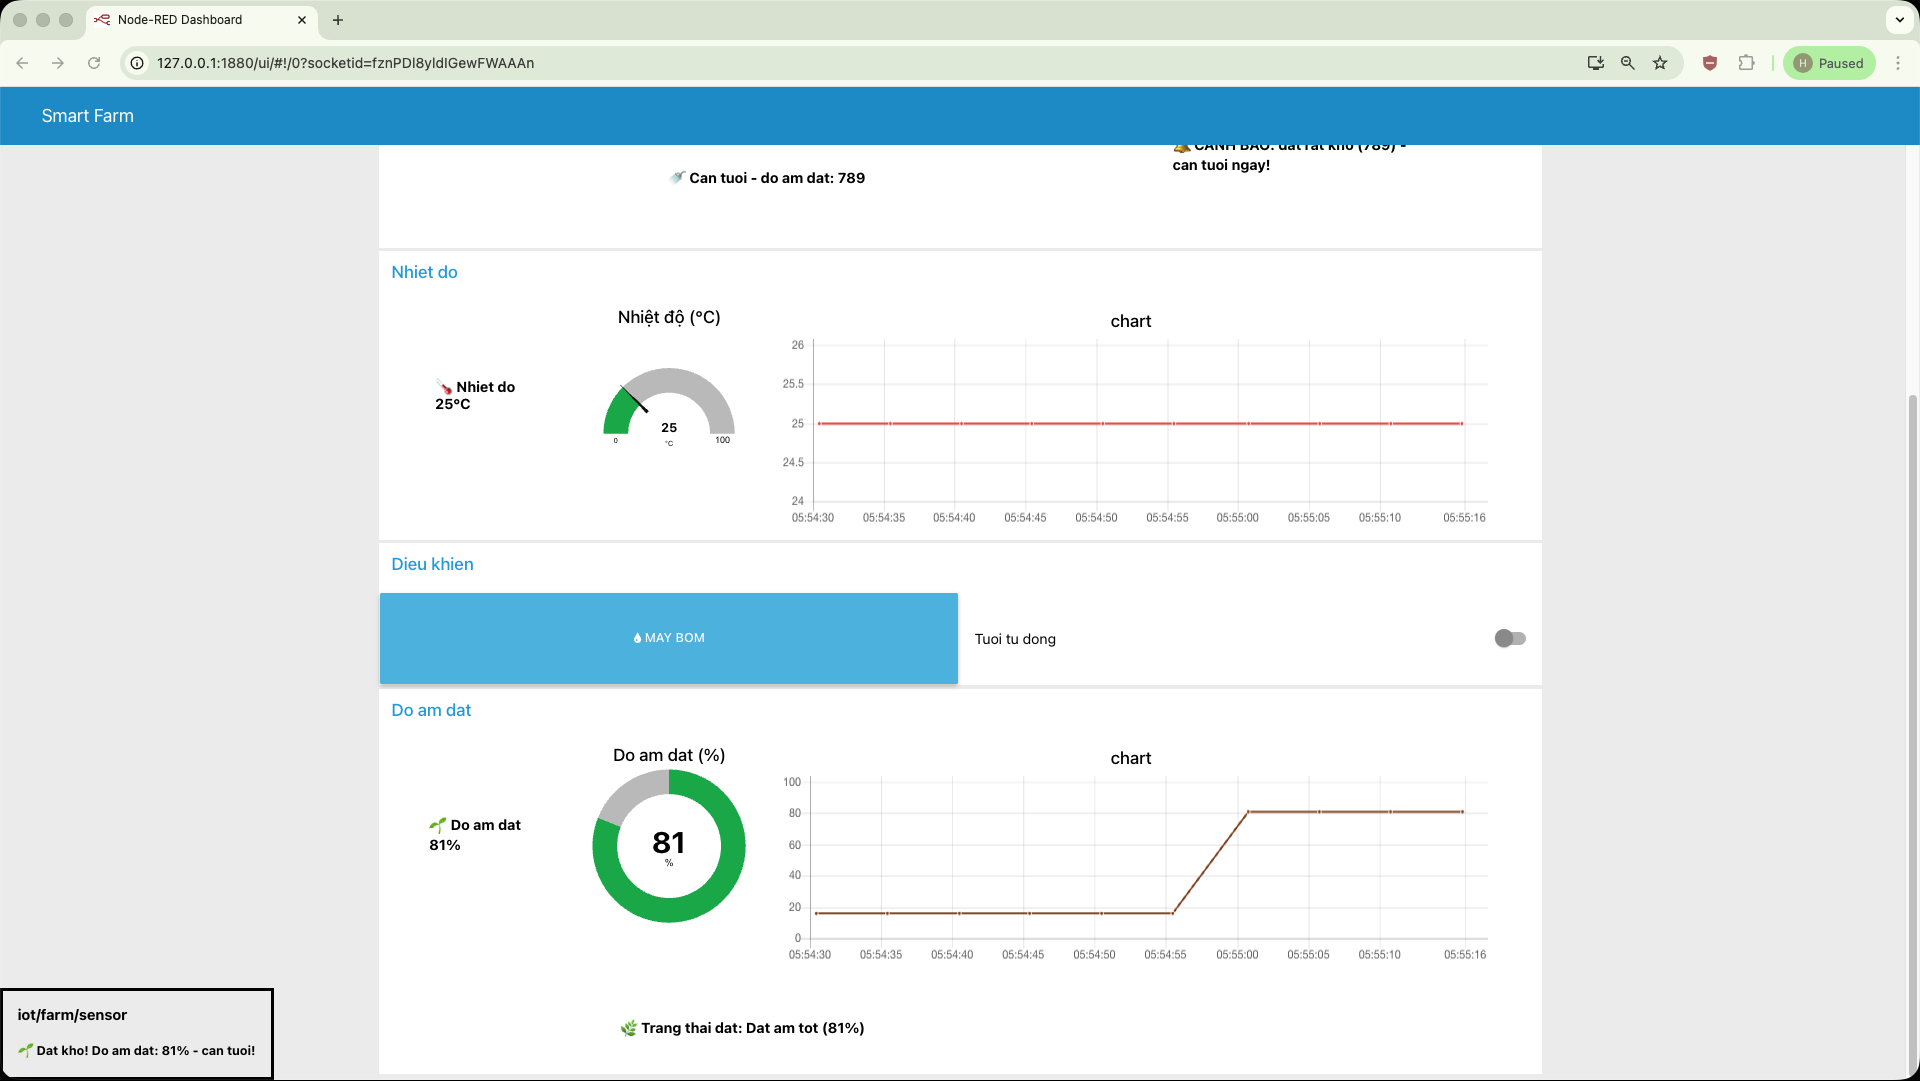
\includegraphics[width=0.9\linewidth]{nodered-dashboard-full-2.png}
  \caption{Minh họa các thông báo cảnh báo và biểu đồ trạng thái trên giao diện Dashboard}
  \label{fig:res-alerts}
\end{figure}

\textbf{Cơ chế điều khiển:} Người dùng có thể thực hiện publish lệnh điều khiển thông qua nút nhấn \textbf{Máy bơm} hoặc kích hoạt chế độ \textbf{Tưới tự động} để hệ thống tự xử lý dựa trên ngưỡng độ ẩm đất.

\textbf{Kết quả mô phỏng:} Môi trường Wokwi phản hồi chính xác các lệnh MQTT gửi đến; đèn LED (giả lập máy bơm) bật/tắt đúng theo yêu cầu và còi báo động hoạt động đồng bộ với trạng thái cảm biến.

\begin{table}[H]
  \centering
  \caption{Tổng hợp các chức năng đã triển khai}
  \label{tbl:chucnang}
  \begin{tabular}{|L{4cm}|C{3cm}|C{4.5cm}|}
    \hline
    \textbf{Chức năng} & \textbf{Trạng thái} & \textbf{Ghi chú} \\
    \hline
    Đọc DHT22 mỗi 5 giây & Hoàn thành & GPIO 4, fallback random khi lỗi \\
    \hline
    Đọc độ ẩm đất (ADC) & Hoàn thành & GPIO 34, potentiometer trên Wokwi \\
    \hline
    Publish/Subscribe MQTT (TLS) & Hoàn thành & Sử dụng giao thức bảo mật cổng 8883 \\
    \hline
    Hiển thị Gauge nhiệt độ & Hoàn thành & 3 vùng màu, min=0, max=100 \\
    \hline
    Hiển thị Gauge độ ẩm KK & Hoàn thành & dạng donut, min=0, max=100 \\
    \hline
    Hiển thị Gauge độ ẩm đất & Hoàn thành & dạng donut, min=0, max=100, 3 vùng màu \\
    \hline
    Biểu đồ line thời gian thực & Hoàn thành & dot=true, removeOlderUnit=3600 \\
    \hline
    Toast cảnh báo nhiệt độ cao & Hoàn thành & Ngưỡng $>$ 35$^\circ$C, 8 giây \\
    \hline
    Toast cảnh báo độ ẩm KK thấp & Hoàn thành & Ngưỡng $<$ 40\%, 8 giây \\
    \hline
    Toast cảnh báo đất khô & Hoàn thành & Ngưỡng soil $<$ 2048, 8 giây \\
    \hline
    Cảnh báo nguy hiểm (đất rất khô) & Hoàn thành & Ngưỡng soil $<$ 1024, hiển thị đỏ \\
    \hline
    Bật bơm thủ công (button) & Hoàn thành & Gửi JSON lên iot/farm/control \\
    \hline
    Tưới tự động (switch) & Hoàn thành & Bật bơm khi ẩm đất $<$ 2048 \\
    \hline
    Cảnh báo buzzer trên ESP32 & Hoàn thành & Phát 2kHz/300ms khi \code{soilRaw < 2048} (firmware) \\
    \hline
    Reconnect Wi-Fi tự động & Hoàn thành & Kiểm tra trong loop() \\
    \hline
    Reconnect MQTT non-blocking & Hoàn thành & Thử lại mỗi 5 giây \\
    \hline
  \end{tabular}
\end{table}

% =============================================================================
% 7. KẾT LUẬN VÀ HƯỚNG PHÁT TRIỂN
% =============================================================================
\section*{CHƯƠNG 7: KẾT LUẬN VÀ HƯỚNG PHÁT TRIỂN}
\phantomsection
\addcontentsline{toc}{section}{CHƯƠNG 7: KẾT LUẬN VÀ HƯỚNG PHÁT TRIỂN}
\label{sec:ch7}
\setcounter{section}{7}
\setcounter{subsection}{0}

\subsection{Các công việc đã hoàn thành}

Qua quá trình triển khai, đề tài đạt các mục tiêu gắn với mã nguồn đính kèm:

Thứ nhất, hệ thống IoT ba tầng hoàn chỉnh: ESP32 + DHT22 + potentiometer (đất) + LED/buzzer; HiveMQ Cloud (TLS); Node-RED Dashboard.

Thứ hai, thu thập và truyền ba thông số mỗi 5 giây qua MQTT (\code{iot/farm/sensor}), JSON chuẩn.

Thứ ba, Dashboard hiển thị gauge, biểu đồ, toast cảnh báo; điều khiển bơm và tưới tự động qua \code{iot/farm/control}.

Thứ tư, mô phỏng Wokwi và sơ đồ EasyEDA minh họa thiết kế.

Hệ thống có thể ứng dụng cho nhà kính, ban công, sân thượng.

\textbf{Ưu điểm:} Chi phí thấp; công cụ mã nguồn mở; MQTT và TLS phù hợp IoT; tách luồng Node-RED dễ bảo trì; reconnect MQTT không chặn \code{loop()}; fallback khi DHT22 trả NaN.

\subsection{Công việc chưa thực hiện và hạn chế}

Chưa tích hợp máy bơm/relay thật (LED mô phỏng); chưa dùng cảm biến độ ẩm đất chuyên dụng; \code{setInsecure()} chỉ phù hợp thử nghiệm; chưa lưu lịch sử ngoài biểu đồ Dashboard; thời gian chạy bơm trên firmware cố định \code{PUMP_DURATION_MS} (chưa dùng \code{duration} từ JSON để tắt theo giây gửi).

\subsection{Hướng phát triển tiếp theo}

Thứ nhất, thay potentiometer bằng cảm biến độ ẩm đất capacitive.

Thứ hai, tích hợp relay và máy bơm nước thực tế; nâng cấp firmware để tự động ngắt bơm dựa trên thời gian (duration) nhận từ bản tin JSON.

Thứ ba, xác thực TLS đầy đủ (CA), bỏ \code{setInsecure()} khi triển khai thực tế.

Thứ tư, InfluxDB/MySQL cho lịch sử và báo cáo.

Thứ năm, ứng dụng di động thay hoặc bổ sung Dashboard.

Thứ sáu, OTA để cập nhật firmware từ xa.

% =============================================================================
% TÀI LIỆU THAM KHẢO — trước phụ lục (theo Phụ lục II: mục 6 rồi mục 7)
% Sau phần Kết luận: không đánh số trang chân trang (rules: chỉ từ Mở đầu đến Kết luận)
% =============================================================================
\newpage
\pagenumbering{gobble}
\section*{TÀI LIỆU THAM KHẢO}
\phantomsection
\addcontentsline{toc}{section}{TÀI LIỆU THAM KHẢO}
\label{sec:tailieu}

\begin{thebibliography}{99}
  \fontsize{13}{17}\selectfont

  \bibitem{esp32} Espressif Systems. \textit{ESP32 Series Datasheet}. Truy cập: \url{https://www.espressif.com/sites/default/files/documentation/esp32_datasheet_en.pdf}.

  \bibitem{nodered} Node-RED. \textit{Node-RED Documentation}. IBM \& others. Truy cập: \url{https://nodered.org/docs/}.

  \bibitem{hivemq} HiveMQ. \textit{HiveMQ Cloud}. Truy cập: \url{https://www.hivemq.com/cloud/}.

  \bibitem{soilmoisture} Seeed Studio. \textit{Capacitive Soil Moisture Sensor}. Truy cập: \url{https://wiki.seeedstudio.com/Capacitive_Soil_Moisture_Sensor/}.

  \bibitem{dht} Adafruit. \textit{DHT sensor library for Arduino}. Truy cập: \url{https://github.com/adafruit/DHT-sensor-library}.

  \bibitem{pubsubclient} Nick O'Leary. \textit{PubSubClient for Arduino}. Truy cập: \url{https://github.com/knolleary/pubsubclient}.

  \bibitem{nodereddash} Node-RED. \textit{node-red-dashboard}. Truy cập: \url{https://flows.nodered.org/node/node-red-dashboard}.

\end{thebibliography}

% =============================================================================
% PHỤ LỤC
% =============================================================================
\newpage

\begin{center}
  {\large\bfseries CÁC PHỤ LỤC}
\end{center}
\vspace{0.5cm}

% ----- PHỤ LỤC A -----
\subsection*{PHỤ LỤC A. Mã nguồn chương trình ESP32}
\phantomsection
\addcontentsline{toc}{subsection}{Phụ lục A. Mã nguồn chương trình ESP32}
\label{sec:pl-a}

\textbf{Lưu ý:} Trước khi nạp firmware, cần cập nhật các thông tin sau trong code: \code{WIFI_SSID} và \code{WIFI_PASSWORD} (tên và mật khẩu Wi-Fi); \code{MQTT_USERNAME} và \code{MQTT_PASSWORD} (tài khoản HiveMQ Cloud). Thông tin xác thực MQTT đã được ẩn trong tài liệu này vì lý do bảo mật.

\IfFileExists{main-src.txt}{%
  \lstinputlisting[
    style=ccode,
    caption={Firmware ESP32 — main.cpp},
    label={lst:pl-arduino}
  ]{main-src.txt}%
}{%
  \textbf{Lỗi:} Không tìm thấy \file{main-src.txt}. Đặt file này cùng thư mục với \file{main.tex}.
}

% ----- PHỤ LỤC B -----
\subsection*{PHỤ LỤC B. Mã nguồn Node-RED (JSON Flow)}
\phantomsection
\addcontentsline{toc}{subsection}{Phụ lục B. Mã nguồn Node-RED (JSON Flow)}
\label{sec:pl-b}

\textbf{Các bước import flow vào Node-RED:}
\begin{enumerate}[label=\arabic*., leftmargin=1.5cm]
  \item Truy cập Node-RED tại \url{http://127.0.0.1:1880}.
  \item Nhấn Menu $\rightarrow$ Import.
  \item Chọn thẻ Clipboard, paste toàn bộ nội dung JSON bên dưới.
  \item Nhấn \textbf{Import} để thêm flow.
  \item Nhấn \textbf{Deploy} (nút đỏ góc phải) để chạy flow.
\end{enumerate}
\textbf{Lưu ý:} Sau khi import, kiểm tra và cập nhật cấu hình node \textbf{mqtt-broker}: hostname, port (8883), username, password phải khớp với tài khoản HiveMQ Cloud đang sử dụng.

\IfFileExists{node-red-flow.txt}{%
  \lstinputlisting[
    style=jcode,
    caption={Node-RED Flow (JSON) — node-red.json},
    label={lst:pl-nodered}
  ]{node-red-flow.txt}%
}{%
  \textbf{Lỗi:} Không tìm thấy \file{node-red-flow.txt}. Đặt file này cùng thư mục với \file{main.tex}.
}

% ----- PHỤ LỤC C -----
\subsection*{PHỤ LỤC C. Mã nguồn sơ đồ Wokwi (JSON)}
\phantomsection
\addcontentsline{toc}{subsection}{Phụ lục C. Mã nguồn sơ đồ Wokwi (JSON)}
\label{sec:pl-c}

\textbf{Các bước mở sơ đồ mạch trên Wokwi:}
\begin{enumerate}[label=\arabic*., leftmargin=1.5cm]
  \item Truy cập \url{https://wokwi.com/}.
  \item Đăng nhập (hoặc tạo tài khoản mới).
  \item Tạo project mới hoặc import file JSON bên dưới.
  \item Nhấn Play để chạy mô phỏng.
\end{enumerate}

\IfFileExists{wokwi-diagram.txt}{%
  \lstinputlisting[
    style=jcode,
    caption={Sơ đồ mạch Wokwi (JSON) — diagram.json},
    label={lst:pl-wokwi}
  ]{wokwi-diagram.txt}%
}{%
  \textbf{Lỗi:} Không tìm thấy \file{wokwi-diagram.txt}. Đặt file này cùng thư mục với \file{main.tex}.
}

% =============================================================================
\end{document}
